\documentclass[master=cws,masteroption=mmc,english]{kulemt}
\setup{title={Design, implementation and evaluation of data integration methods for biomedical cancer data},
	author={Michiel Ruelens},
	promotor={Prof.\,dr.\,ir.\ Roel Wuyts \& Prof. Olivier Gevaert},
	assessor={Ir.\,W. Eetveel\and W. Eetrest},
	assistant={Ir.\ A.~Assistent \and D.~Vriend}}
% De volgende \setup mag verwijderd worden als geen fiche gewenst is.
\setup{filingcard,
	translatedtitle={Design, implementatie en evaluatie van data integratie methoden voor biomedische kankergegevens},
	udc=621.3,
	shortabstract={Hier komt een heel bondig abstract van hooguit 500
		woorden. \LaTeX\ commando's mogen hier gebruikt worden. Blanco lijnen
		(of het commando \texttt{\string\pa r}) zijn wel niet toegelaten!
		\endgraf \lipsum[2]}}
% Verwijder de "%" op de volgende lijn als je de kaft wil afdrukken
%\setup{coverpageonly}
% Verwijder de "%" op de volgende lijn als je enkel de eerste pagina's wil
% afdrukken en de rest bv. via Word aanmaken.
%\setup{frontpagesonly}

% Kies de fonts voor de gewone tekst, bv. Latin Modern
\setup{font=lm}

% Hier kun je dan nog andere pakketten laden of eigen definities voorzien
\usepackage{amsmath}
\usepackage{bm}
\usepackage[]{algorithm2e}
\usepackage[table]{xcolor}

% Tenslotte wordt hyperref gebruikt voor pdf bestanden.
% Dit mag verwijderd worden voor de af te drukken versie.
\usepackage[pdfusetitle,colorlinks,plainpages=false]{hyperref}

% Colors
\definecolor{lightgray}{gray}{0.95}
%%%%%%%
% Om wat tekst te genereren wordt hier het lipsum pakket gebruikt.
% Bij een echte masterproef heb je dit natuurlijk nooit nodig!
\IfFileExists{lipsum.sty}%
{\usepackage{lipsum}\setlipsumdefault{11-13}}%
{\newcommand{\lipsum}[1][11-13]{\par Hier komt wat tekst: lipsum ##1.\par}}
%%%%%%%

%\includeonly{chap-n}
\begin{document}
	
	\begin{preface}
		I would like to thank everybody who kept me busy the last year,
		especially my promotor and my assistants. I would also like to thank the
		jury for reading the text. My sincere gratitude also goes to my wive and
		the rest of my family.
	\end{preface}
	
	\tableofcontents*
	
	\begin{abstract}
		The \texttt{abstract} environment contains a more extensive overview of
		the work. But it should be limited to one page.
		
		\lipsum[1]
	\end{abstract}
	
	\begin{abstract*}
		In dit \texttt{abstract} environment wordt een al dan niet uitgebreide
		Nederlandse samenvatting van het werk gegeven.
		Wanneer de tekst voor een Nederlandstalige master in het Engels wordt
		geschreven, wordt hier normaal een uitgebreide samenvatting verwacht,
		bijvoorbeeld een tiental bladzijden. 
		
		\lipsum[1]
	\end{abstract*}
	
	% Een lijst van figuren en tabellen is optioneel
	%\listoffigures
	%\listoftables
	% Bij een beperkt aantal figuren en tabellen gebruik je liever het volgende:
	\listoffiguresandtables
	% De lijst van symbolen is eveneens optioneel.
	% Deze lijst moet wel manueel aangemaakt worden, bv. als volgt:
	\chapter{List of Abbreviations and Symbols}
	\section*{Abbreviations}
	\begin{flushleft}
		\renewcommand{\arraystretch}{1.1}
		\begin{tabularx}{\textwidth}{@{}p{12mm}X@{}}
			LoG   & Laplacian-of-Gaussian \\
			MSE   & Mean Square error \\
			PSNR  & Peak Signal-to-Noise ratio \\
		\end{tabularx}
	\end{flushleft}
	\section*{Symbols}
	\begin{flushleft}
		\renewcommand{\arraystretch}{1.1}
		\begin{tabularx}{\textwidth}{@{}p{12mm}X@{}}
			42    & ``The Answer to the Ultimate Question of Life, the Universe,
			and Everything'' according to \cite{h2g2} \\
			$c$   & Speed of light \\
			$E$   & Energy \\
			$m$   & Mass \\
			$\pi$ & The number pi \\
		\end{tabularx}
	\end{flushleft}
	
	% Nu begint de eigenlijke tekst
	\mainmatter
	
	\chapter{Introduction}
\label{cha:intro}
The first contains a general introduction to the work. The goals are
defined and the modus operandi is explained.

\section{The need for data integration methods}

\section{Goals}

\section{Modus operandi}

%%% Local Variables: 
%%% mode: latex
%%% TeX-master: "thesis"
%%% End: 

	\chapter{Generalized Linear Models}
\label{cha:glm}

\section{Introduction}
\label{sec:glm-introduction}
In this chapter I will explain the concepts of generalized linear models. This term indicates a generalization of simple linear regression that allows for a wide range of output variables. First I will go over the basics of linear models, gradually building up to the definition of generalized linear models. Next, I will describe what actual data looks like and how a model is computed from it. After that I will tackle the more recent innovation of regularization that will greatly improve our previous models by exploiting the bias-variance trade-off to reduce overfitting. Lastly I will outline the validation method that will be used to test the performance of the models.

\section{Classical linear models}
\label{sec:glm-classicallinearmodels}
When we think of classical linear models, we can imagine a set of numeric explanatory (or input) variables and a numerical dependent (or output) variable. By making a linear combination of the explanatory variables we attempt to estimate a value for the dependent variable. Depending on the type of dependent variable the linear method gets a different name. In the following sections I will outline several of them.

\subsection{Linear Regression}
The simplest version of a linear model is called linear regression. In this case the input variables are combined using a linear combination, and the result of this calculation is immediately used as the final estimate. Imagine we have a dataset of size N where each sample has M explanatory variables. Then we can write linear regression as:\\
\begin{equation}
\begin{split}
y_{n} = \sum_{i=1}^{M}w_{i}x_{in} = \bm{w^{T}x}   \qquad for\ n=1..N
\end{split}
\end{equation}
where
\begin{itemize}
	\item $y_{n}$ is the output for sample $n$
	\item $w_{i}$ is the model parameter (co\"effici\"ent) for explanatory variable $i$
	\item $x_{in}$ is the value for explanatory variable $i$ for sample $n$
	\item $\bm{w^{T}x}$ is the vector notation for the inner product of $\bm{w}$ and $\bm{x}$
\end{itemize}
For the other linear methods we will define a function each time that is applied to the result of the linear combination. We could do the same for linear regression and say that the applied function is the identity function. A schema for this computation is shown on figure \ref{fig:glm-linear-regression}.\\
\begin{figure}
	\centering
	\includegraphics[scale=.6]{images/linear_regression.png}
	\caption{Schema for linear regression}
	\label{fig:glm-linear-regression}
\end{figure}
\subsection{Linear Classification}
The next method is called linear classification. The difference with linear regression is that we have a different type of output variable. In a classification task we want to predict a class from a list of potential classes. For instance, we could try to predict whether tomorrow will be a sunny day or not. Notice that there are only 2 possible outcomes: 'sunny' or 'not sunny' and we could represent these outcomes as 0 and 1 in our model. This form would be called binary classification because we have 2 possible classes. It is very easy to extend this method to multi-class classification.\\
The computation in this method starts out exactly the same, combining the input variables using a linear combination. Next, we have to define a threshold to indicate which examples belong to one class or another. In the case of binary classification we would define 1 threshold, and if the result of the linear combination is higher than the threshold we would predict one class. If it is lower, we would predict the other class. The function used here would be called a sign function, which maps real values onto one of 2 possible outcomes. We could represent this computation with the following formula: 
\begin{equation}
\begin{split}
y_{n} =
\begin{cases} 
0 & if\ \bm{w^{T}x} \leq t \\
1 & if\ \bm{w^{T}x} > t 
\end{cases}
\qquad for\ n=1..N
\end{split}
\end{equation}
where
\begin{itemize}
	\item $y_{n}$ is the output for sample $n$
	\item $\bm{w^{T}x}$ is the vector notation for the inner product of $\bm{w}$ and $\bm{x}$
	\item $t$ is the classification threshold
\end{itemize}
A schema for this computation is shown on figure \ref{fig:glm-linear-classification}.
\begin{figure}
	\centering
	\includegraphics[scale=.6]{images/linear_classification.png}
	\caption{Schema for linear classification}
	\label{fig:glm-linear-classification}
\end{figure}
\subsection{Logistic Regression}
The third method I want to present is called logistic regression. In this case, the output variable we want to predict comes from a binomial distribution. This means that they are the result of a probabilistic event. An example would be tossing a coin and checking whether the result is heads or tails. While the outcome is binary (heads or tails) we know that there is an underlying probability for the coin to be heads or tails, and we would like to know this probability. \\
The idea is still the same. We will make a linear combination of the input variables. However this time we will use a logistic function to produce our estimate. The logistic function is a function that maps real numbers onto the range $[0,1]$. This result can then be interpreted as an estimate for the probability. We could represent logistic regression mathematically as:
\begin{equation}
\begin{split}
y_{n} = \theta(\sum_{i=1}^{M}w_{i}x_{in})= \theta(\bm{w^{T}x}) \qquad for\ n=1..N
\end{split}
\end{equation}
where
\begin{itemize}
	\item $y_{n}$ is the output for sample $n$
	\item $w_{i}$ is the model parameter (co\"effici\"ent) for explanatory variable $i$
	\item $x_{in}$ is the value for explanatory variable $i$ for sample $n$
	\item $\bm{w^{T}x}$ is the vector notation for the inner product of $\bm{w}$ and $\bm{x}$
	\item $\theta(x)$ is a logistic function, also called a sigmoid function. An example sigmoid function is $\frac{e^{x}}{1+e^{x}}$
\end{itemize}
\begin{figure}
	\centering
	\includegraphics[scale=.6]{images/logistic_regression.png}
	\caption{Schema for logistic regression}
	\label{fig:glm-logistic-regression}
\end{figure}
A schema for this computation is shown on figure \ref{fig:glm-logistic-regression}.
The logistic regression method is the one that will be most widely used throughout this thesis.

\section{Training a model}
\label{sec:glm-trainingamodel}
In order to understand the integration strategies that will be explained later on, it is useful to know how exactly the models come to be. This section will explain what the input data for our linear models actually looks like, and how we get from this data to a model that we can use for future predictions.
\subsection{The data}

The data we use consists of two parts: the input data, which can be seen as a matrix where the columns are the explanatory variables and each row is an example. And secondly the output data, which can be seen as a vector where each value indicates the value of the dependent variable for a single example. \\
It is easy to see that the length of the output vector has to be equal to the amount of rows in the input matrix, indeed there should be one output value for each example. This amount is often called the size of the dataset and we would like it to be as big as possible. Especially when we are dealing with a large number of explanatory variables, it is essential to have a reasonable amount of examples aswell. This will be discussed in more detail in section \ref{sec:glm-overfitting} on overfitting. 

\subsection{Gradient descent}
In this section I will explain how we get from the input data to the model. The idea here is that we have some error measure. The error measure is a sort of rating for our current model as it indicates how big the mistakes are that our current model makes. Once we have a way of computing this error, we can try to minimize the error to obtain our 'best' possible model.
\subsubsection{Error measure}
In logistic regression the error measure we use is called the cross-entropy error. The formula for this error is the following:
$$
	E_{in}(w) = \frac{1}{N}\sum_{n=1}^{N}ln(1+e^{-y_{n}w^{T}x_{n}})
$$
where
\begin{itemize}
	\item $x_{n}$ is the vector of values for the explanatory variables for example $n$.
	\item $y_{n}$ is the value of the dependent variable for example $n$.
	\item $w^T$ is the transpose of the weights vector. These are the parameters of our model that we can adjust.
	\item $N$ is the size of our dataset.
	\item $E_{in}(w)$ is the in-sample error. This is the cross-entropy error that we make on the examples in our dataset. It is a function of the weights $w$.
\end{itemize}
We can intuitively see that this is a reasonable error measure. It is an averaged sum over all examples, where for each example we compute an individual error made on that example. Notice that $w^{T}x_{n}$ is the linear combination of the input variables that our current model suggests. This is the prediction that our current model would make for example $n$ and is a real valued number. On the other hand $y_{n}$ is the actual correct prediction for example $n$ and has a value of 0 or 1. If the signs of $w^{T}x_{n}$ and $y_{n}$ agree then our current model actually makes a correct prediction for this example. We can see that in this case the exponential becomes close to 0, making our error for example $n$ very small, as we would expect. If however their signs are opposite, the exponential becomes larger as our incorrect prediction becomes larger. This in turn will increase the error, again as we would expect. Thus we can see that if we were to minimize this error, we are moving towards a model that tries to make correct predictions.
\subsubsection{The gradient descent method}
When trying to minimize a function, a general approach would be to try and compute the derivative of the function, and find the value where this derivative equals zero. In the case of linear regression it is actually possible to compute this minimum in one step. More details about this can be found in appendix //TODO ADD AND REFERENCE APPENDIX. \\
In the case of logistic regression however it is not possible to find an analytic solution to this problem. The best we can do is put ourselves somewhere on the error surface and try to move towards the minimum in small steps. This is called an iterative approach. Remember that our error function looks like this:
$$
E_{in}(w) = \frac{1}{N}\sum_{n=1}^{N}ln(1+e^{-y_{n}w^{T}x_{n}})
$$
We can now compute its derivative with respect to $w$:
$$
\nabla E_{in}(w) = -\frac{1}{N}\sum_{n=1}^{N}\frac{y_{n}x_{n}}{1+e^{y_{n}w^{T}x_{n}}}
$$
The problem is to find the set of weights $w$ for which the derivative becomes 0 (or that minimizes the error). We can start out with an initial set of weights $w(0)$ and then iteratively update these weights so we move towards the minimum. Let's call the direction in which we update our weights $v$. The update we make to $w$ then becomes:
$$
w(t+1) = w(t) + \eta v
$$
where
\begin{itemize}
	\item $w(t+1)$ are the updated weights for this iteration.
	\item $w(t)$ are the current weights before we make a move.
	\item $v$ is a unit vector pointing in the direction we want to move.
	\item $\eta$ is a number that indicates how big the move is that we make, also called the step size.
\end{itemize}
Remember that the gradient of a function at a certain point always points towards the steepest slope upwards. In our case we would like to find the minimum, so it is a good idea to move our weights in the direction of steepest descent. The direction $v$ that we are moving towards then becomes the normalized opposite direction of the gradient:
$$
v = -\frac{\nabla E_{in}(w(t))}{\lVert\nabla E_{in}(w(t))\rVert}
$$
We can now summarize the gradient descent method as follows: \\ \\
\begin{algorithm}[H]
	\KwData{x, y}
	initialize weights w(0) \\
	\While{Stopcondition is not met}{
		Compute gradient $\nabla E_{in}(w(t))$\\
		Compute update direction $v$ \\
		Update weights $w(t+1) = w(t) + \eta v$
	}
\caption{Gradient Descent algorithm}
\end{algorithm}
There are two more non-trivial issues in this computation: the initialization of the weights and the stopcondition. \\ \\
Weight initialization is sometimes a very tricky thing to do, in the case of logistic regression however it is acceptable to set $w(0)$ equal to the zero-vector as this corresponds to no correlation between any of the input variables and the output variable, and the result of the sigmoid function would be 0.5 or 50\% meaning the model has no preference for either outcome.\\ \\
The stopcondition however is a bigger issue and usually the way to go here is to make a combination of several stop criteria. One criteria would be to simply limit the amount of iterations to a fixed number. This could avoid endlessly overfitting. Another criteria is to set up a target error we want to achieve (a small number), and stop when we have reached this target. This however raises the question of picking the target error, and this is mostly an application dependent choice. \\ \\
In the version of logistic regression explained here, it can however be shown that the error surface we are dealing with is a very nice convex surface. This makes it very easy to find its minimum and we don't need very complex initialization and stopping criteria to get good results. In other machine learning methods however these surfaces aren't always as nice, and the issue of local minima versus global minima becomes a big deal. There has been much research on this topic however and many sophisticated methods have been developped to deal with this issue.

\section{Overfitting}
\label{sec:glm-overfitting}
Now that we have established a method of computing our models, it is time to deal with an issue known as overfitting. Overfitting points to the fact that there are several mechanisms at work when we are building a model that prevent us from reaching the perfect model (a model that predicts correctly at all times). These mechanisms essentially originate from noise and uncertainty in many aspects of the learning process (the input data, choice of model, choice of algorithm, ...). We can however try to decompose this noise into several components and then attempt to influence them by making changes to our model computation. I will present two ways in which overfitting can be tackled: regularization and validation.

\subsection{The problem of overfitting}
Let's introduce some notation. From now on I will refer to the notion of 'in-sample error' or in symbolic notation $E_{in}$ as the error that a model makes on the examples in our training set. The training set consists of the examples that were used to train (compute) the model in the first place. \\
Similarly I will define 'out-of-sample error' or $E_{out}$ as the error we make on examples that were not used for training the model. Notice that $E_{in}$ is something we could compute because we have access to the training data, but $E_{out}$ is a quantity we cannot exactly compute but we could try to estimate it if we have some examples left that we did not use for training. Notice also that it is $E_{in}$ that we minimize during our model computation, but it is $E_{out}$ that we actually want to minimize! Indeed, $E_{out}$ corresponds to the error that we get when we are going to deploy our model in practice and use it on examples we have never seen before. We can do this because we believe that $E_{in}$ tracks $E_{out}$ to a certain degree. And thus if we manage to minimize $E_{in}$ we also minimize $E_{out}$ to some extent. \\
We can only speak of overfitting when we are comparing two models. We say that one model, call it model A, is overfitting with respect to another model, model B, when model A managed to get a lower $E_{in}$ than model B, but model B has a lower $E_{out}$. \\
Another way of looking at it is during the learning process. Let's have model A be the model that we computed when we started from model B and performed one more iteration of the training algorithm. Thus model A is 'more trained' than model B. Now let's suppose model A is overfitting:
\begin{align}
E_{in}^{modelA} < E_{in}^{modelB} \\
E_{out}^{modelA} > E_{out}^{modelB}
\end{align}
The additional iteration has decreased the in-sample error, and thus we are able to fit our training data better, but the out-of-sample error has increased, meaning that our model doesn't generalize as well to other examples outside the training set. This means that we are actually fitting our training data too well, while we are not really getting a better grasp of the underlying pattern that we wish to learn. We are overfitting the training data.\\
\subsection{The bias and variance trade-off}
There are several ways of looking at overfitting and pointing out its origins. I will introduce the notions of bias and variance and how they can describe the noise in our system. \\
\subsubsection{Average hypothesis}
First, let me explain the playing field. We are in a situation of learning, where we are given a set of examples that are produced by some target function $f$. It is this target function $f$ that we wish to learn (or in other words model). In order to do this we have to decide on the type of functions that we will use to model. In machine learning this is called the hypothesis set. It is the set of all functions that we consider possible candidates to fit our target $f$. And we will use the examples $x$ in our dataset $D$ to decide which hypothesis we will pick. \\
Next, let's introduce the notion of average hypothesis $\bar{h}$. Imagine we have a very large number of datasets. For each of these datasets we apply the learning process and we will pick a certain hypothesis $h$ from our hypothesis set. The average hypothesis is then equal to the average of all the hypothesis' just learned. Or in a formula:
$$
\bar{h} = \mathbf{E}_{D}[h^{(D)}]
$$
where
\begin{itemize}
	\item $\bar{h}$ is the average hypothesis.
	\item $\mathbf{E}_{D}$ is the expected value over an infinite number of datasets
	\item $h^{(D)}$ is the hypothesis that was learned for a specific dataset D
\end{itemize}
We can also look at this average hypothesis as sort of the best we can do with the given hypothesis set. Indeed, when we imagine having an infinite number of datasets we would end up cancelling out much of the variation in the learned hypothesis' and end up with a very good one. \\
\subsubsection{Bias}
We can now define the bias as the distance between the average hypothesis $\bar{h}$ and our target function $f$.
$$
bias = (\bar{h} - f)^{2}
$$
We can see the bias as an error we make due to our own choices. Namely our choice of hypothesis set. If we choose a very simple hypothesis set, we cannot expect to be able to find a fit for a very complex function. The target function simply isn't contained in our hypothesis set. There exists no function in our hypothesis set that exactly fits our target. \\
Therefore we introduced the notion of average hypothesis. We can view this as the best we can do given our current hypothesis set, and the distance to the target is what we call the bias.
\subsubsection{Variance}
This however is not the full story. In a real learning situation we generally never find this average hypothesis, because remember it required a large amount (or even infinite amount) of datasets. We never have this luxury! In reality we always have only one dataset and that is all we can use to navigate through the hypothesis set. This is where the notion of variance comes in. We can define variance as the error we get from not having the best hypothesis possible in our hypothesis set. Or in other words as the distance between the hypothesis set that we actually found by learning from our dataset and the average hypothesis.
$$
variance = (h^{(D)} - \bar{h})^{2}
$$
Error due to variance mainly comes from two sources: the first is our finite dataset, the second is the complexity of the hypothesis set.\\
In reality we are given a dataset of $N$ examples and that's all you've got. Most of the time this dataset is not sufficient to find the best hypothesis and thus there will be a variance error made. \\
Secondly, as we increase the complexity of the hypothesis set, it becomes increasingly difficult to navigate through this set. There are simply many more hypothesis to choose from. Again this makes it harder for our learning process to find the optimal hypothesis and as such will introduce a variance error.
\subsubsection{The tradeoff}
Having both bias and variance defined we can see that they are not disconnected, there is a tradeoff. If we look purely at bias we could think that simply choosing a super complex hypothesis set is always optimal. Indeed our bias will be zero since the target function will always be inside our hypothesis set. \\
However, an increasingly complex hypothesis set makes it harder to actually find the optimal hypothesis. We know that the optimal hypothesis is there, but we just cannot find it. The take-away message here is that we have to choose a hypothesis set complexity based on the resources that we have. In this case the resource is our dataset. The larger the dataset that we can learn from, the more complex hypothesis sets we can afford, and the better our results will be. But there is no gain in choosing overly complex hypothesis sets when you don't have the resources to afford them. This will simply cause you to find hypothesis' that fit your training data very well (imagine fitting 3 datapoints with a 7th order polynomial, you would get an exact fit) but this model will not generalize to anything in the real world, it is a complete overfit.
\section{Regularization}
\label{sec:glm-regularization}
Now that we have the concepts of bias and variance, let's use this information to try and improve our models. The first method is called regularization. In very simple terms this method will add a very small amount of bias in order to greatly decrease the amount of variance, reducing the overall error we make.
\subsection{Adding bias}
Remember that bias is defined as the distance between the average (or best) hypothesis $\bar{h}$ and our target function $f$. Adding bias effectively means we are going to make another choice, which will impact the average hypothesis. The choice we are about to introduce is based on the following observation: when confronted with a set of similarly performing models, the simplest model is usually the best. Or in other words we should try to prefer simple models over very complex ones. \\
This observation does not have a mathematical proof, it is rather an observation from experience and reason. One good argument is the fact that noise is usually of high frequency. Meaning that distortions of our dataset (for instance measurement errors) will often be very scattered and random, while the underlying pattern that really makes up the data will be rather smooth. A similar argument can be made for the error due to bias, when we choose a hypothesis set that does not contain the target function, the error due to bias will be mostly random and of high frequency. Therefore if we want to reduce the impact of this noise in our final model, we should prefer models that are not able to fit these high frequencies exactly. Lastly we can remark that if we look at our current understanding of nature (let's say at a larger scale), systems almost always have smooth transitions. The most important laws of nature that we find are all written down in small, simple formulas. Nature doesn't work with instantaneous changes (high frequency), but rather it has smooth functions that govern the basic principle, and then it adds random noise and fluctuations on top of it. This principle is what we try to extrapolate here to machine learning.\\
Thus, the choice we will make is that we will prefer simple models over complex ones by adding a constraint to the weights.
\subsection{Regularization types}
There are many kinds of constraints that we could add to the weights and, depending on the constraint we choose, the regularization gets a different name and it will have a different effect. One of the most famous regularizers is called ridge or weight-decay. The constraint for this regularizer is the following:
$$
\sum_{i=1}^{N}w_{i}^{2} \leq C
$$
where
\begin{itemize}
	\item $w_{i}$ is the weight (model parameter) for the i'th explanatory variable.
	\item $C$ is the constraint value
\end{itemize}
Using this regularizer will result in a preference for models with smaller weights. This keeps certain weights from getting out of control. This form of regularization is also often called the $L_{2}$ penalty. \\
Another popular regularizer is called the lasso penalty (or $L_{1}$ penalty). The constraint in this case is:
$$
\sum_{i=1}^{N}\lvert w_{i}\rvert \leq C
$$
In addition to keeping the weights small, this form of regularization also performs parameter selection. This means that instead of just keeping the weights small it will also prefer to make weights actually zero. This will cause the resulting model to have fewer parameters, but the parameters that do survive the penalty are sure to be very important. This regularizer is often used when there is a huge number of explanatory variables, and we wish to find only those that are really descriptive. Later in the thesis I will use datasets that contain gene expression information about cancer patients, these datasets often have thousands of explanatory variables and will provide a good example for using the lasso regularization. \\
The last form of regularizer I wish to demonstrate is called the elastic net penalty. This regularizer is simply a linear combination of the ridge and lasso penalties and provides a way of balancing the two. It has the following constraint:
$$
\alpha \sum_{i=1}^{N}w_{i}^{2} + (1-\alpha)\sum_{i=1}^{N}\lvert w_{i}\rvert \leq C
$$
\subsection{Lambda}
Using a regularizer introduces a constraint, this means that we now have to deal with a constrained optimization problem which is much harder to solve than an unconstrained problem. Fortunately, through some clever mathematics it is possible to convert the constrained minimization problem to an unconstrained one by incorporating the regularization constraint in the formula for the error itself. //TODO ADD APPENDIX WITH FULL DERIVATION OR NOT ... The formula for the error with regularization then becomes:
$$
E_{in}(w) = \frac{1}{N}\sum_{n=1}^{N}e(x_{n},y_{n},w)+\lambda R(w)
$$
where
\begin{itemize}
	\item $E_{in}(w)$ is the in-sample error.
	\item $e(x_{n},y_{n},w)$ is the individual error made on example n. In the case of logistic regression this would be a cross-entropy error term $ln(1+e^{-y_{n}w^{T}x_{n}})$.
	\item $\lambda$ is the regularization parameter that will be explained below.
	\item $R(w)$ is the regularization term dependent on the type of regularization used. For instance: $\sum_{i=1}^{N}\lvert w_{i}\rvert$ for lasso, $\sum_{i=1}^{N}w_{i}^{2}$ for ridge, ...
	\item $x_{n}$ is the n'th sample in the dataset.
	\item $y_{n}$ is the outcome for the n'th sample in the dataset.
	\item $w$ is the vector of weights, our model parameters that we are trying to find.
\end{itemize}
Notice that we now again have an error measure that we want to minimize, and it is an unconstrained optimization problem. The important new part is $\lambda$. This is the amount of regularization we want to use. It is a new form for the constraint constant $C$ that was earlier introduced in the types of regularization. The higher $\lambda$ the tighter the constraint (lower $C$) and vice versa. The value of $\lambda$ will prove to be critical in getting good models. The way to calculate it is through validation.
\section{Validation}
\label{sec:glm-validation}
In this section I will explain the method of validation which is used to estimate the out-of-sample error. I will first explain the issue of sample size and then present a method to work around this limitation.
\subsection{The sample size dilemma}
Remember that when we are training a model we use the in-sample error to navigate the hypothesis space. We do this because we believe that the in-sample error is a valid surrogate for the out-of-sample error (which is the error we actually want to minimize).
A valid question to ask is: why don't we just estimate the out-of-sample error and minimize it directly? Consider the following situation: \\
We are given a dataset of $N$ samples. I will use $K$ samples of the dataset to train my model, this leaves me with $N-K$ samples that are not used for training. Since $K$ samples were used for training, if I would compute the error the model makes on these samples I would be computing the in-sample error. If I want to estimate the out-of-sample error I have to use the $N-K$ samples that were not used for training. This sample set of $N-K$ samples if often called the validation set.\\
We can now make the following observations:
\begin{itemize}
	\item The larger we choose K, the more samples are available for training and thus the better our model can be (due to lower variance!)
	\item The larger we choose K, the less accurate our out-of-sample error estimate is, because we have fewer datapoints for the estimation
\end{itemize}
So now it is clear that we have a tradeoff to make. We would like K to be as large as possible so that we have a large amount of samples to train a model from. On the other hand we would like K to be as small as possible so that we have enough samples to estimate the out-of-sample error. The solution to this apparent contradiction will be cross-validation.
\subsection{Cross-validation}
Cross-validation is a technique that allows us to have plenty of samples left for training, while still getting a pretty good estimate for the out-of-sample error. The method is as follows: divide the dataset of $N$ samples into $K$ equal parts (often called folds). Each fold now has $N/K$ samples. Train a model on $K-1$ folds and use the remaining fold to estimate the out-of-sample error. Repeat this process $K$ times, one time for each of the $K$ folds, each time leaving out a different fold. In the end we have $K$ estimates of the out-of-sample error and we can average them to get a final result.\\ \\
Notice that we are really using all samples for validation and training, but never both at the same time. It feels a bit like cheating, but in practice this method works wonderfully. Validation is often used to determine parameters of the learning process, for instance the $\lambda$ parameter for regularization. We simply try several values for $\lambda$, compute the out-of-sample error using validation, and pick the $\lambda$ that gives the lowest error. Once we have decided this $\lambda$ we can then train a model on the full dataset of $N$ points and use the $\lambda$ we have just calculated to be optimal. \\ \\
We have to remark however that when we use validation to calculate a value for $\lambda$ as described above, we are really using the validation to help train the model. In this case we can no longer make the statement that the validation samples are not used for training. This is called data pollution. We are using the same data to train training parameters aswell as training the model itself and it is obvious that this will give rise to additional correlations in the data. However in practice it is generally accepted that if you use this technique to decide on just a few learning parameters (often just $\lambda$), and you have a big enough dataset, the data pollution is minimal and the results and estimates you get are still reliable. \\ \\
Cross-validation is not only used to estimate learning parameters. It can also be used to simply test the performance of the model. In this case the fold that is not used for training is usually not called a validation set, but rather a test set. Because samples in this set will be used to test the models performance. 

\section{Conclusion}
\label{sec:glm-conclusion}
We have now covered the basis of Generalized Linear Models. We have described the gradient descent method that we can use to navigate the hypothesis space by minimizing an error function. We have seen that overfitting is a serious issue that is caused by noise at different levels of the learning process. We have broken down this noise into bias and variance and shown that we can have an impact on this process. We can use regularization to add a slight bias in order to greatly decrease the error due to variance and we have based this on the principle that we should prefer simple and smooth models. Lastly we have covered the method of validation. A method that we can use to estimate the out-of-sample error and which gives us the ability to choose learning parameters like $\lambda$ and also test the performance of our model.

%%% Local Variables: 
%%% mode: latex
%%% TeX-master: "thesis"
%%% End: 

	\chapter{Cox proportional hazards models}
\label{cha:cox}

\section{Introduction}
\label{sec:cox-introduction}
This chapter explains the cox proportional hazards model\cite{simon2011regularization}\cite{tibshirani1997lasso}\cite{wikicox}. This is a model that is used in survival analysis. The first section explains what survival analysis means and how it is different from the generalized linear models. Next we will define what the proportional hazards assumption is and lastly we will show kaplan-meier survival curves and how we can compute them from hazard functions.

\section{Survival analysis}
\label{sec:cox-survival-analysis}
Survival analysis points to the fact that the outcome variables are time-to-event datapoints. A common example in biomedical research would be the time between the start of a patients treatment and the time of death. Note however that not all patients have to die in order to be useful in a survival analysis. A second outcome variable is used to indicate whether the patient survived until the end of the study, or not. This (often binary) variable is called the censoring variable. \\ \\
A typical outcome in survival analysis is thus represented by two vectors: a time to event vector and a censoring vector. An example is shown in table \ref{tab:cox-example-outcome}.
\begin{table}
	\centering
	\begin{tabular}{cc}
		\toprule
		Time (days) & Censor\\
		\midrule
		249 & 1 \\
		345 & 1 \\
		152 & 1 \\
		452 & 0 \\
		120 & 1 \\
		... & ... \\
		\bottomrule
	\end{tabular}
	\caption{Example outcomes for survival data}
	\label{tab:cox-example-outcome}
\end{table}
The idea of survival analysis is now to find a pattern between a set of explanatory variables and the time-to-event. A common term used in survival analysis is hazard, meaning 'risk of the event occurring'. A resulting model from survival analysis usually contains two components. The first component is a $\lambda_{0}(t)$ baseline hazard function. This function describes how the risk of the event occurring changes with time, assuming there is no influence from any of the explanatory variables. The second component describes the influence of each explanatory variable on the hazard. This brings us to the notion of proportional hazards.

\section{Cox proportional hazards model}
\label{sec:cox-proportional-hazards-model}
\subsection{Proportional hazards condition}
The proportional hazards condition means that we assume that hazard ratios are independent of time. A hazard ratio is the relative risk between two entities (patients). Furthermore the condition states that changes in the explanatory variables have an exponential effect on the hazard. The following paragraphs explain these statements in more detail.\\ \\
If we assume the proportional hazards condition to be true then this gives us the opportunity to estimate the effect of explanatory variables without dealing with the underlying baseline hazard function. This was an observation made by Sir David Cox\cite{cox1972life}, hence the name of the model. We can represent the cox model as follows:
\begin{equation}
\begin{split}
\lambda_{i}(t) = \lambda_{0}(t)e^{X_{i1}\beta_{1} + ... + X_{iN}\beta_{N}}
\end{split}
\end{equation}
where
\begin{itemize}
	\item $\lambda_{i}(t)$ is the hazard for patient i at time t.
	\item $\lambda_{0}(t)$ is the baseline hazard at time t.
	\item $X_{i1} ... X_{iN}$ are the values of the explanatory variables for patient i.
	\item $\beta_{1} ... \beta_{N}$ are the values of the coefficients for each explanatory variable.
\end{itemize}
Now, let's look at relative risks between two patients:
\begin{equation}
\begin{split}
\frac{\lambda_{i}(t)}{\lambda_{j}(t)} 
= \frac{\lambda_{0}(t)e^{X_{i1}\beta_{1} + ... + X_{iN}\beta_{N}}}{\lambda_{0}(t)e^{X_{j1}\beta_{1} + ... + X_{jN}\beta_{N}}}
= e^{(X_{i1}-X_{j1})\beta_{1} + ... + (X_{iN}-X_{jN})\beta_{N}}
\end{split}
\end{equation}
This quantity is called the hazard ratio. Notice that this ratio does not depend on time. This means that if at the start of the study a patient has twice the risk of the event occurring compared to another patient, it will have twice the risk at any other time aswell. It's risk remains proportional, independent of time. \\ \\
We can also compute the effect on the hazard for a unit increase in an explanatory variable $X_{j}$. The subscripts i to indicate the patients have been omitted since this is independent of a specific patient. The hazard ratio then becomes:
\begin{equation}
\begin{split}
\frac{\lambda(t|X_{j}+1)}{\lambda(t|X_{j})} = e^{(X_{j}+1-X_{j})\beta_{j}} = e^{\beta_{j}}
\end{split}
\end{equation}
It is directly given by the exponential of the coefficient for the explanatory variable. This reflects the proportional hazards assumption that hazard ratios do not depend on time and that explanatory variables have an exponential effect on the hazard.
\subsection{Using the hazard ratio}
The proportional hazards assumption allows us to compute relative risks or hazard ratios without knowing the actual baseline hazard function. Knowing just relative ratios can be very useful however. Imagine the following scenario: we want to test if a certain drug increases the survivability of patients with a specific disease. We randomly give half of the patients the actual drug, the other half receives a placebo (or nothing at all). Performing a survival analysis using a cox model then allows us to compute the ratio of the hazards for the two groups. The coefficient for the explanatory variable that indicates which patients received the drug and which did not then tells us the effect of the drug on the hazard. We could then make a statement such as: "Taking the drug tends to half the risk of the event occurring (at any time)." This is obviously a useful result to support further research or development for the drug.

\subsection{Kaplan-Meier survival curves}
Kaplan-Meier survival curves\cite{goel2010understanding} are often used in survival analysis. These curves show the probability of surviving up to any point t. It is thus a declining curve starting from 1 at $t=0$. An example curve is shown on figure \ref{fig:cox-example-kaplan-meier}.
\begin{figure}
	\centering
	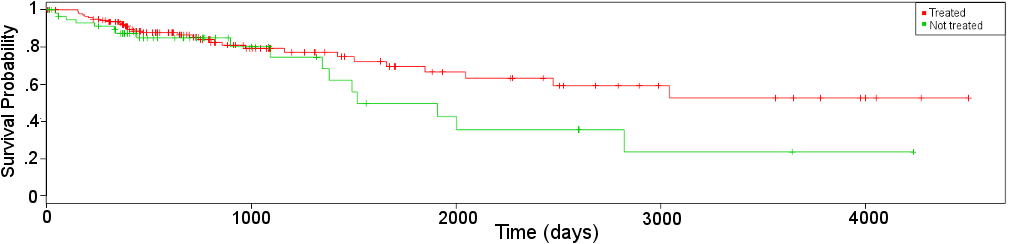
\includegraphics[scale=0.4]{images/example_kaplan_meier_curve}
	\caption{Example Kaplan-Meier survival curve. Red and green lines represent survival probabilities for treated and untreated patient-groups respectively.}
	\label{fig:cox-example-kaplan-meier}
\end{figure}
In formula notation we could write this as:
\begin{equation}
\begin{split}
S(t) = P(T > t)
\end{split}
\end{equation}
where
\begin{itemize}
	\item $S(t)$ is the survival function
	\item $P(x)$ means 'the probability of x'
	\item $T$ is the observed event time (e.g. death)
	\item $t$ is the time variable
\end{itemize}
\subsubsection{Linking hazard to survival}
Creating a kaplan-meier survival curve based on the outcome vectors (time and censoring) is very straightforward to do, it is simply a visual representation of the event occurring at certain times. However when we create a model that tries to explain these outcomes from explanatory variables we end up with a hazard function. In order to create survival curves we have to link this hazard function to the survival function\cite{survivalmodels}. Recall the hazard function $\lambda(t)$ from section \ref{sec:cox-proportional-hazards-model}. We could write this function in a similar probabilistic notation as we did for the survival function:
\begin{equation}
\begin{split}
\lambda(t) = \lim\limits_{\delta\rightarrow0}\frac{P(t < T \leq t+\delta | T  > t)}{\delta}
\end{split}
\end{equation}
this is really just the definition of hazard: the risk of the event happening at time t is defined as the event happening during an infinitesimal timeframe after time t, given that the event has not happened yet up to time t. As we take the limit $\delta\rightarrow0$ this becomes an instantaneous hazard. We can now apply the conditional probability rule $P(A|B) = \frac{P(A \cap B)}{P(B)}$ to get:
\begin{equation}
\begin{split}
\label{eq:cox-hazard}
\lambda(t) &= \lim\limits_{\delta\rightarrow0}\frac{P(t < T \leq t+\delta \cap t < T)}{\delta}\frac{1}{P(T>t)} \\
&= \lim\limits_{\delta\rightarrow0}\frac{P(t < T \leq t+\delta)}{\delta}\frac{1}{S(t)} \\
&= \lim\limits_{\delta\rightarrow0}\frac{P(t < T) - P(t+\delta\leq T)}{\delta}\frac{1}{S(t)} \\
&= -\lim\limits_{\delta\rightarrow0}\frac{P(t+\delta\leq T) - P(t < T)}{\delta}\frac{1}{S(t)} \\
&= -\frac{\partial S(t)}{\partial t}\frac{1}{S(t)} \\
&= -\frac{S'(t)}{S(t)}
\end{split}
\end{equation}
Let's look at this result in an intuitive way. Assume the event we are talking about is dying. The hazard function then tells me what the risk is of dying at time $t$. Equation \ref{eq:cox-hazard} tells us that this is equal to $-\frac{S'(t)}{S(t)}$. There are three parts to explain here:
\begin{itemize}
	\item $\frac{1}{S(t)}$: The first thing we have to do is survive up to time $t$. Otherwise it makes no sense to ask what the risk of dying at time $t$ is. The survival function tells us how probable it is to survive up to time $t$ so dividing by this quantity exactly provides what we need. If $S(t)$ is large, then this means many people survive up to time $t$ and so the risk is low. If $S(t)$ is small then few people actually survive up to time $t$ and thus the risk of having to survive up to this point gets bigger.
	\item $S'(t)$: Now that we have survived up to time $t$, we need to calculate the risk of dying at this point in time. Remember that the survival curve declines whenever people die at certain points in time. The slope of this function therefore tells us how many people die at that time $t$. If $S'(t)$ is very large, it means that many people die here. The risk of dying thus becomes large.
	\item The hazard is supposed to be a positive quantity. Since the survival function is a strictly declining curve (people usually don't resurrect from the dead), $S'(t)$ is negative. Therefore we need the minus sign to end up with a positive result.
\end{itemize}
Next, using the chain rule, we can observe that
\begin{equation}
\begin{split}
\label{eq:cox-survival}
\frac{\partial log(S(t))}{\partial t} = \frac{S'(t)}{S(t)}
\end{split}
\end{equation}
and thus combining equations \ref{eq:cox-hazard} and \ref{eq:cox-survival}:
\begin{equation}
\begin{split}
\lambda(t) &= -\frac{\partial log(S(t))}{\partial t}
\end{split}
\end{equation}
\begin{equation}
\begin{split}
\label{eq:cox-int-hazard}
\int_{0}^{t}\lambda(t)dt &= \int_{0}^{t}-\frac{\partial log(S(t))}{\partial t}dt
\end{split}
\end{equation}
The left hand side of equation \ref{eq:cox-int-hazard} is called the cumulative hazard fuction and often denoted $\Lambda(t)$. We can then write:
\begin{equation}
\begin{split}
\Lambda(t) &= -log(S(t))
\end{split}
\end{equation}
\begin{equation}
\begin{split}
\label{eq:cox-survival-hazard-link}
S(t) &= e^{-\Lambda(t)}
\end{split}
\end{equation}
Equation \ref{eq:cox-survival-hazard-link} allows us to relate the survival function to the hazard function. This allows us to create survival curves for any form of hazard function. The only thing that is left to do is to define the baseline hazard function, because otherwise we could not compute the integral in $\Lambda(t)$ . Usually an estimator based on likelihood is used to estimate the baseline hazard function. There are many forms available for this estimator\cite{royston2011estimating}, but we will not go into any more detail here.

\section{Conclusion}
\label{sec:cox-conclusion}
In this chapter we have explained the cox proportional hazards method. We have shown that it is used for survival analysis, where the targets are time and censoring variables. We have explained the proportional hazards assumption and shown its implications. Lastly we have shown how we can compute survival curves using the Kaplan-Meier method and we have shown a relationship between the hazard function and the survival function.
%%% Local Variables: 
%%% mode: latex
%%% TeX-master: "thesis"
%%% End: 

	\chapter{Integration Strategies}
\label{cha:integration}

\section{Introduction}
\label{sec:integration-introduction}
Now that we have established a firm understanding of the methods we will use to create predictive models, it is time to turn our attention to the integration step. In this chapter we will present three different integration strategies. We will start by providing a description of the datasets that we will use to build our models, followed by the integration strategies that show how we can combine these datasets to create predictive models. The first strategy is called early integration and is based on concatenation of datasets. The second strategy is called late integration which is based on ensemble learning. The last strategy is intermediate integration which makes extensive use of the variable selection present in the lasso regularization(\ref{sec:glm-regularization}).

\section{Description of the data}
\label{sec:integration-description}
In order to integrate the datasets, they have to adhere to a number of requirements. Suppose we have a set of D datasets, each dataset can be represented by a matrix where the rows are the samples and the columns are the explanatory variables. Each dataset can have different explanatory variables, but they all need to have rows that can be linked across datasets, for instance using a unique patient identifier. Let me give a concrete example: imagine we have a set of 200 cancer patients. Each of these patients has had images taken of the cancer by different machines: an MRI scan, a PET scan, ... and they also had a bloodtest done measuring different prote\"{i}ne levels in the blood (an ELISA test). Each of these methods will yield a dataset: one for each imaging scan and one for the blood test. The explanatory variables are obviously different for each dataset: the imaging datasets will have image features like blobs and pixel intensities, while the bloodtest will have values that represent the prote\"{i}ne levels in the blood. Each dataset will however have a single row per patient, uniquely identified by that patients ID. This is not true in the case of missing data (e.g. a patient missed his MRI scan appointment). But there are ways of dealing with this: we can try to estimate the missing values using clustering techniques, or we can simply leave the patients with missing data out of the study. \\ \\
Now that we have our input data, we need a target function (dependent variable). In the example case this could be whether the patient fully recovers from the treatment or not. This variable is supposed to have a binomial distribution and thus we could use logistic regression to try and estimate this variable. The task of integration is now the following: how do we combine the samples across the different datasets to come up with a predictive model that uses the information in all the datasets? In the following sections we will present three ways to do this: the early integration method which is concatenation, the late integration method that is based on an ensemble of models, and the intermediate integration method that takes advantage of variable selection present in the lasso regularization.

\section{Early integration}
\label{sec:integration-early}
The first integration method is called early integration. In this method we are simply going to concatenate the data for each sample. Figure \ref{fig:integration-early} shows the schema for early integration of data sources. A new large dataset is constructed by concatenating the individual datasets by matching sample. The number of explanatory variables is now equal to the sum of explanatory variables of all individual datasets. This integrated dataset can then be used to train a predictive model using techniques seen in previous chapters (\ref{cha:glm},\ref{cha:cox}).
\begin{figure}
	\centering
	\includegraphics[scale=.8]{images/early_integration}
	\caption{Scheme for early integration}
	\label{fig:integration-early}
\end{figure}
\section{Late integration}
\label{sec:integration-late}
In late integration, as the name suggests, we will combine the different datasets at the end of the learning process. The schema for late integration is shown on figure \ref{fig:integration-late}. First, a model is learned for each dataset individually. This gives rise to $D$ different models. To reuse the example from section \ref{sec:integration-description}, there will be a model for MRI data, PET data, etc. When we want to predict an outcome for a new sample (patient) we will present each model with the corresponding input from the patient. Each model will then compute an output and these are combined using a linear combination. If we have no preference for any model we could simply compute the average output. This average would then be our final output for the integrated model. In this case we cannot represent the final model by some model parameters (weights) but rather we have to view the full set of $D$ models as well as the linear combination we chose as the full integrated model. \\ \\
There is an analogy between late integration and the ensemble averaging technique in machine learning. Ensemble learning \cite{dietterich2002ensemble}\cite{dietterich2000ensemble}\cite{wikiensemble} means that instead of just building one model for a dataset, we build several models for the same dataset and then average their outcomes. Late integration takes this idea but applies it to a set of data sources instead of just one. \\ \\
The thought behind this model is that we try to learn as much as possible from each dataset individually, before we combine them. An example of this is that the variable selection by the lasso regularization (section \ref{insec:glm-lasso}) now has the opportunity to select the best variables for each dataset individually. While in the case of early integration, all the variables from the datasets are competing against each other at the same time to make it into the final model.
\begin{figure}
	\centering
	\includegraphics[scale=.8]{images/late_integration}
	\caption{Scheme for late integration}
	\label{fig:integration-late}
\end{figure}
\section{Intermediate integration}
\label{sec:integration-intermediate}
Intermediate integration is a novel integration technique that tries to take advantage of the variable selection when using a lasso penalty. The schema for intermediate integration is shown on figure \ref{fig:integration-intermediate}. It starts out the same way as late integration, for each dataset we compute an individual model. However, instead of using the output of these models we will simply look at the variables that were chosen by each model to be informative. We will then go back to the original datasets and extract only those explanatory variables and concatenate them together into a new integrated dataset. Lastly, we use this integrated dataset to learn a final model. \\ \\
The intermediate integration can be seen as a two-step learning process. First we preprocess the datasets by computing individual models and we extract only the informative variables. Then we will train our final model on the reduced dataset. This is very advantageous if the initial datasets have a huge amount of explanatory variables, as the preprocessing step will reduce this amount drastically while still keeping as much useful information as possible.
\begin{figure}
	\centering
	\includegraphics[scale=.8]{images/intermediate_integration}
	\caption{Scheme for intermediate integration}
	\label{fig:integration-intermediate}
\end{figure}
\section{Conclusion}
\label{sec:integration-conclusion}
In this chapter we have shown the issue of large and high-dimensional datasets that we are currently facing. We have presented three different strategies to deal with this issue. The early integration method is the na\"{i}ve method that simply concatenates the datasets together. The late integration method uses an analogous technique to ensemble learning in order to extract as much information as possible. Lastly, the intermediate integration technique introduces a two-step learning method that takes advantage of variable selection to reduce the dimensionality of the datasets.
%%% Local Variables: 
%%% mode: latex
%%% TeX-master: "thesis"
%%% End: 

	\chapter{Tool for automated evaluation}
\label{cha:tool}

\section{Introduction}
\label{sec:tool-introduction}

\section{Technologies}
\label{sec:tool-technologies}

\section{Demonstration}
\label{sec:tool-demonstration}

\section{Conclusion}
\label{sec:tool-conclusion}

%%% Local Variables: 
%%% mode: latex
%%% TeX-master: "thesis"
%%% End: 

	\chapter{Tool for automated evaluation}
\label{cha:tool}

\section{Introduction}
\label{sec:tool-introduction}
In the previous chapter we have shown that different integration strategies do make a difference for the performance of the resulting model. In order to facilitate future research on this topic, we have developed a tool that allows anyone to very easily compute all the integrated models and compare them.
\section{Technologies}
\label{sec:tool-technologies}
To develop this tool we needed a programming language that provided a lot of support for statistical algorithms, and we also wanted to create a very user-friendly interface to make an abstraction of the underlying machine learning methods.
\subsection{The R language}
The language we used to create the tool is R. R is a very popular language for statistical research as it provides many state-of-the-art algorithms in statistics. R has a huge repository with packages for all kinds of purposes. The package that we used to compute models is glmnet \cite{glmnetvignette}. It is developed by researchers at the Stanford University and provides very fast implementations to compute the generalized linear models explained in chapter \ref{cha:glm}. 
\subsection{Web interface}
I wanted to offer a very easy-to-use interface to the application. Therefore we chose to work with shiny \cite{shiny}. Shiny is a framework for R that allows you to create a web-based front-end (using html, css, javascript, ...) that can also run R code in the back-end. This allows the creating of very interactive web applications that can run the powerful statistical analyses available in R.
\section{Demonstration}
\label{sec:tool-demonstration}
The tool is divided into three sections: an input section where the user can upload their datasets, a section that computes and evaluates models for each dataset individually, and an integration section where all of the integrated models, explained in chapter \ref{cha:integration}, can be computed and evaluated.
\subsubsection{The input tab}
The input tab allows the user to either use a preloaded dataset or upload their own datasets to the application. It is possible to define multiple dependent variables in one file, the tool then gives you the option to select which variable has to be modeled. \\ \\
When datasets are uploaded, the tool gives a small overview of the dimensions of each dataset so the user can verify everything works correctly. Figures \ref{fig:tool-input} and \ref{fig:tool-input2} show the input page where a user has uploaded some datasets.
\begin{figure}
	\centering
	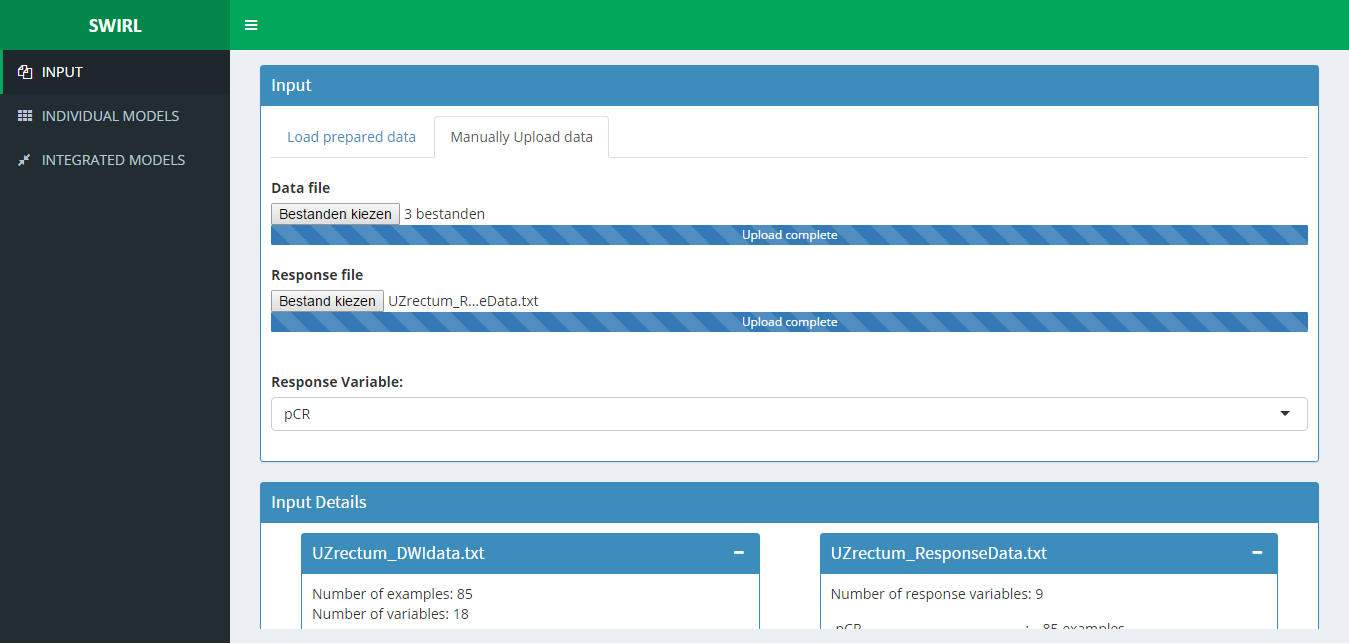
\includegraphics[scale=.3]{images/tool_input_1}
	\caption{The input tab of the tool}
	\label{fig:tool-input}
\end{figure}
\begin{figure}
	\centering
	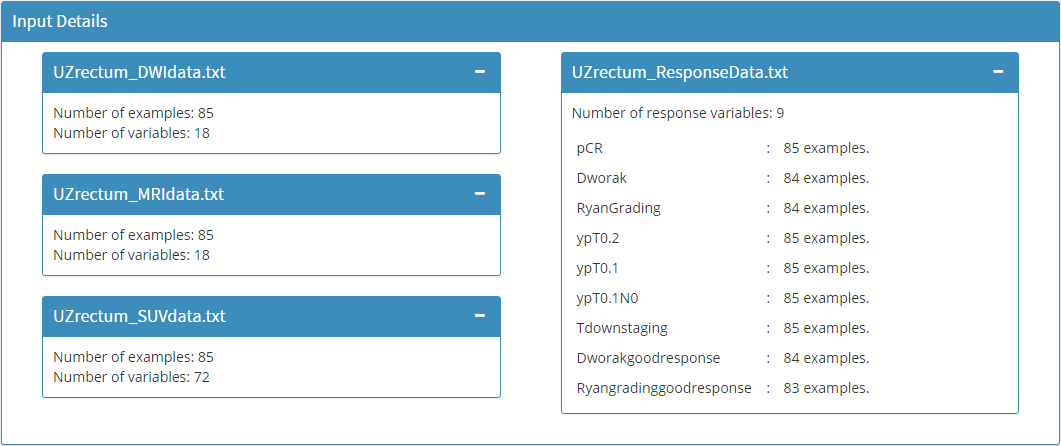
\includegraphics[scale=.4]{images/tool_input_overview}
	\caption{Example input overview. The boxes on the left show explanatory variable dataset dimensions, the box on the right shows the possible dependent variables.}
	\label{fig:tool-input2}
\end{figure}
\subsubsection{The individual models tab}
Once a user has uploaded their datasets they can compute a model for each dataset individually. The tool will give a concise overview of the model parameters for each model, and show an evaluation of the model. In case of logistic regression, the evaluation would be a ROC curve (explained in section \ref{sec:evaluation-logisticregression}). Notice that the evaluation is interactive: the user can use the slider to see the performance metrics for different thresholds. Figure \ref{fig:tool-model} shows an example model description. Figure \ref{fig:tool-roc} shows an example ROC curve.
\begin{figure}
	\centering
	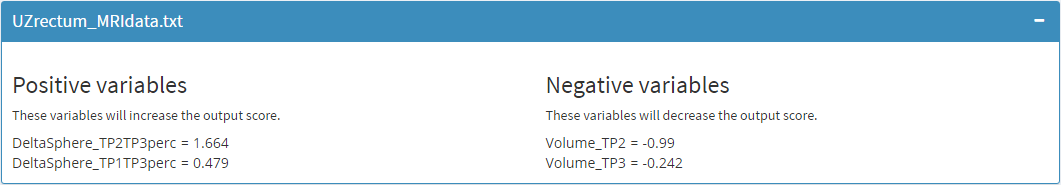
\includegraphics[scale=.4]{images/tool_model_mri}
	\caption{An example model description showing the coefficients for the variables in the model separated by their sign.}
	\label{fig:tool-model}
\end{figure}
\begin{figure}
	\centering
	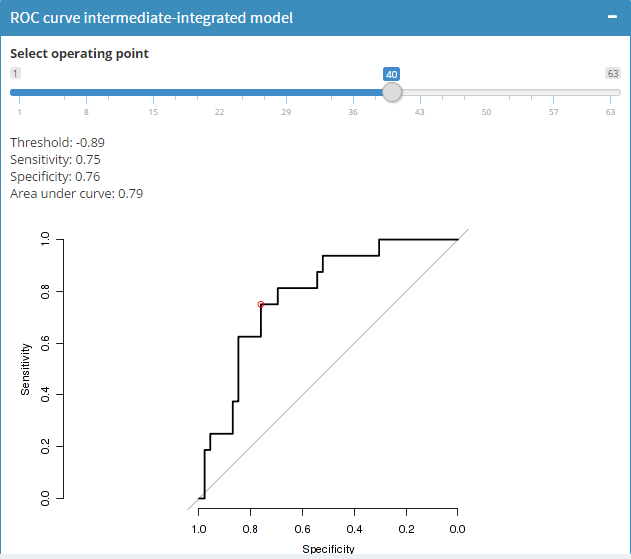
\includegraphics[scale=.65]{images/tool_auc}
	\caption{An example interactive ROC curve. The slider on top allows the user to vary the threshold. The plot interactively adjusts itself to the chosen threshold.}
	\label{fig:tool-roc}
\end{figure}
\subsubsection{The integration tab}
The integration tab is the most important part of the application, as it allows the user to compute and evaluate integrated models for their datasets. The integration tab is further split up into early-, late- and intermediate integration tabs. Each tab allows the user to compute and evaluate its respective integration method. The results will look exactly the same as shown for the individual models tab, as can be seen on figures \ref{fig:tool-model} and \ref{fig:tool-roc}.

\section{Conclusion}
\label{sec:tool-conclusion}
To make further research easier we have made an interactive web-based tool. The tool allows users to compute and evaluate all integration strategies explained earlier. It currently supports logistic regression models and cox proportional hazard models. The back-end uses the statistical language R and the glmnet package to compute the models. The front-end is purely web-based and this is made possible by the Shiny framework.

%%% Local Variables: 
%%% mode: latex
%%% TeX-master: "thesis"
%%% End: 

	% ... en zo verder tot
	\chapter{Conclusion}
\label{cha:conclusion}
The final chapter contains the overall conclusion. It also contains
suggestions for future work and industrial applications.

\lipsum[1-7]

%%% Local Variables: 
%%% mode: latex
%%% TeX-master: "thesis"
%%% End: 

	
	% Indien er bijlagen zijn:
	\appendixpage*          % indien gewenst
	\appendix
	\chapter{Cross-entropy error derivation}
\label{app:cross-entropy}
In this appendix I will explain where the cross-entropy error measure for logistic regression comes from. First I will explain the setting and make sure all used symbols are clear. Next I will introduce the notion of likelihood. And lastly I will derive the cross-entropy error function based on the likelihood idea.

\section{The setting of logistic regression}
Remember that in logistic regression we are trying to estimate a probability. The output variable $y$ is a binary variable that comes from an underlying binomial distribution, think of tossing a coin and observing heads or tails. Let's call the target function that we wish to fit $f(x)$. This function defines the probability of finding outcome $y$ when given input $x$. We could write this in a formula:
\begin{equation}
\begin{split}
P(y | x) =
\begin{cases} 
f(x) & for\ y=1 \\
1-f(x) & for\ y=-1 
\end{cases}
\end{split}
\end{equation}
Here $P(y | x)$ is the probability of finding $y$ given $x$. It is equal to $f(x)$ if the event occurred and, since it is a binary event, it is equal to $1-f(x)$ if the event didn't occur. The statement that we are making in logistic regression is that we can find a linear combination of the input variables and pass it through a sigmoid function to approximate $f(x)$. Finding in this case means defining the weights of the linear combination. We will call the final set of weights the final hypothesis $h(x)$.
\begin{equation}
\begin{split}
h(x) = \theta(\bm{w^{T}x}) \approx f(x)
\end{split}
\end{equation}
\section{Likelihood}
The notion of likelihood is basically an inversion of the usual thought process. What we usually think of when talking about supervised learning is: what is the probability of finding an outcome $y$ given the data $x$. Here we are going to invert the statement and define likelihood as: if $h(x) = f(x)$ how likely is it to see the data $x$ given the output $y$. Or in a formula:
\begin{equation}
\begin{split}
P(y | x) =
\begin{cases} 
h(x) & for\ y=1 \\
1-h(x) & for\ y=-1 
\end{cases}
\end{split}
\end{equation}
Notice that we now assume that $h(x)$ is generating the outcomes instead of $f(x)$.
Remember that we defined $h(x) = \theta(\bm{w^{T}x})$, and thus: 
\begin{equation}
\begin{split}
P(y | x) =
\begin{cases} 
\theta(\bm{w^{T}x}) & for\ y=1 \\
1-\theta(\bm{w^{T}x}) & for\ y=-1 
\end{cases}
\end{split}
\end{equation}
A useful property of the sigmoid function is that $\theta(-x) = 1-\theta(x)$. We can use this fact to get rid of the cases in the formula, because if we change the second case by $\theta(-x)$ we get:
\begin{equation}
\begin{split}
P(y | x) =
\begin{cases} 
\theta(\bm{w^{T}x}) & for\ y=1 \\
\theta(\bm{-w^{T}x}) & for\ y=-1 
\end{cases}
\end{split}
\end{equation}
Now notice that the sign in each case corresponds to the value of $y$. We could multiply each case by the corresponding value of $y$ to obtain:
\begin{equation}
\begin{split}
P(y | x) = \theta(y\bm{w^{T}x})
\end{split}
\end{equation}
Now we define the likelihood of the dataset $D$ by multiplying the likelihood of each sample:
\begin{equation}
\begin{split}
Likelihood(D) = \prod_{n=1}^{N}P(y_{n}|x_{n}) = \prod_{n=1}^{N}\theta(y_{n}\bm{w^{T}x_{n}})
\end{split}
\end{equation}
We now want to maximize the above likelihood of the dataset, given that the hypothesis $h(x)$ is indeed the correct target.

\section{Lorem 51}
\lipsum[51]

%%% Local Variables: 
%%% mode: latex
%%% TeX-master: "thesis"
%%% End: 

	% ... en zo verder tot
	\begin{abstract*}
\section{Introductie}
\label{cha:D:intro}
\subsection{De nood aan data integratie methoden}
Recente technologische vooruitgang zorgt ervoor dat datasets groter en groter worden. Dit is een trend die in vele gebieden merkbaar is, ook in het biomedische veld. Met grotere datasets bedoelen we dat de datasets zowel in aantal variabelen toenemen, als in het aantal datapunten. Het toenemende aantal variabelen is vooral te wijten aan de technologie. We zijn op het punt gekomen dat we relatief goedkoop ieders DNA kunnen uitlezen. Als we dan weten dat een gemiddelde persoon zo'n 20.000 tot 25.000 genen heeft die coderen voor prote\"inen, dan is het niet moeilijk om je in te beelden dat datasets duizenden variabelen bevatten. Een ander voorbeeld vinden we in de vooruitgang van beeldvormingsinstrumenten. Elk ziekenhuis beschikt tegenwoordig over talloze gigantisch geavanceerde scanners (MRI, PET, ...) die uiterst nauwkeurige afbeeldingen kunnen maken. Uit deze afbeeldingen kunnen heel wat variabelen worden afgeleid. Dit zijn slechts twee voorbeelden die aantonen dat het aantal variabelen enorm groeit. Naast deze groei zien we ook dat het aantal datapunten in de datasets stijgt. Ook dit heeft meerdere oorzaken. Een eerste oorzaak is simpelweg het feit dat we nu meer gegevens kunnen opslaan dan vroeger. Het is niet langer ongewoon om gigabytes of zelfs petabytes aan gegevens bij te houden. Een tweede oorzaak is dat onderzoekers over heel de wereld ijveren tot openstelling van gegevens. Als alle onderzoekers hun gegevens publiek delen met de hele wereld, dan heeft iedereen gewoonweg meer datapunten om te analyzeren, wat uiteindelijk de algemene vooruitgang zou stimuleren. \\ \\
De groei van datasets brengt echter ook problemen met zich mee, we moeten namelijk zoeken naar technieken om al deze gegevens van verschillende bronnen op de beste manier met elkaar te combineren tot een coherent systeem.

\subsection{Doel en werkwijze}
Het doel van dit thesis is om enkele integratie strategie\"en te ontwikkelen en aan te tonen dat deze strategie\"en een impact hebben op de performantie van predictieve modellen. In plaats van predictieve modellen te bouwen voor individuele datasets zullen we dus proberen om meerdere datasets te combineren en 1 predictief model te bouwen dat alle gegevens gebruikt en dat een betere performantie biedt dan alle andere individuele modellen. Om dit te doen is het belangrijk dat we eerst goed begrijpen wat een predictief model is en hoe we er een kunnen opbouwen. Het eerste hoofdstuk legt uit wat we bedoelen met predictieve modellen en stelt het eerste type voor: het logistieke regressie model. Het volgende hoofdstuk geeft een tweede type van predictief model dat we overlevingsmodellen noemen. Specifiek zullen we ons focussen op het cox model. Vervolgens zullen we de verschillende integratie strategie\"en voorstellen. Om aan te tonen dat deze strategie\"en effectief een impact hebben op de performantie van de modellen zullen we twee concrete case-studies tonen. De eerste case-studie zal logistieke regressie gebruiken om predictieve modellen te bouwen, gebruik makend van alle integratie strategie\"en. De tweede case-studie zal hetzelfde doen voor de survival modellen. In beide case-studies zullen alle modellen ge\"evalueerd worden met geschikte technieken. \\ \\
Om het hele proces te ondersteunen hebben we een interactieve applicatie ontwikkeld die in staat is om de performantie van predictieve modellen te evalueren. Dit liet ons toe om de twee case-studies op te bouwen, maar het vormt ook een platform voor toekomstig onderzoek.

\section{Predictieve modellen}
\label{cha:D:predictieve-modellen}

\subsection{Introductie}
\label{sec:D:pm-introductie}
In dit hoofdstuk leggen we uit wat een predictief model inhoudt en hoe deze worden opgebouwd. We zullen hiervoor twee concrete voorbeelden gebruiken: logistieke regressie en cox survival modellen. Verder leggen we ook het concept van regularisatie uit, dit zal belangrijk blijken in het volgende hoofdstuk over integratie strategie\"en. Tenslotte zullen we ook kort uitleggen wat validatie inhoudt.

\subsection{Wat is een predictief model?}
\label{sec:D:pm}
Een predictief model is een relatie tussen input variabelen en een doelfunctie (doel variabele). De taak van een predictief model is om een waarde te voorspellen voor de doelfunctie, gegeven een set van waarden voor de input variabelen. Bijvoorbeeld: we kunnen een predictief model bouwen dat de relatie probeert voor te stellen tussen een datum en de gemiddelde temperatuur op die dag. De input is hier de datum, de doelfunctie (of output) is de gemiddelde temperatuur voor die dag. We kunnen ons inbeelden dat er tussen deze twee variabelen een verband bestaat. Een datum ergens in de zomer zal namelijk een relatief hoge gemiddelde temperatuur opleveren, en een dag in de winter een relatief lage temperatuur. We weten dit omdat we jarenlang ervaring hebben opgebouwd en ons hebben gerealizeerd dat het in de zomer normaal warm is en in de winter koud. Dit is precies wat we proberen te vatten met een predictief model, het onderliggende patroon. En de manier om daartoe te komen is door ervaring op te bouwen. Op eenzelfde manier gaan we proberen het model ervaring te laten opbouwen, we noemen dit dan 'het model trainen'. We gaan het model voorbeelden tonen van wat we willen dat het model leert, en het model zal hieruit leren en intern een representatie opbouwen om zijn kennis voor te stellen. In het eerder gegeven voorbeeld zouden we, om het model te trainen, een hele lijst met data en de corresponderende gemiddelde temperatuur voor die dag tonen aan het model, dit noemen we de training set. Het model zal dan intern een representatie opbouwen van zijn kennis en als alles goed verloopt zal deze representatie inderdaad weergeven dat het in de zomer normaal warmer is en in de winter normaal kouder. Welke representatie het model intern gebruikt is een keuze die we zelf maken, en hangt af van het type van patronen dat we willen representeren en dus van de relatie die we denken dat er bestaat tussen de input en de doelfunctie. Er zijn talloze representaties mogelijk, in dit thesis focussen we ons op lineaire representaties. Dit wil zeggen dat we veronderstellen dat we een lineaire combinatie kunnen maken van de input variabelen, en daarmee accuraat de doelfunctie kunnen benaderen. Afhankelijk van het type van de doelfunctie die we willen benaderen zijn hier echter nog verschillende methoden voor, in de volgende secties bekijken we twee concrete voorbeelden: logistieke regressie en cox modellen.

\subsection{Logistieke regressie}
\label{subsec:D:pm-logistieke-regressie}
In logistieke regressie maken we twee veronderstellingen. De eerste is dat er een lineair verband bestaat tussen de input variabelen en de doelfunctie. De tweede is dat, in de training set, de waarden van de doelfunctie het resultaat zijn van een binomiaalverdeling. Denk hierbij bijvoorbeeld aan het genezen of niet-genezen van een kankerpati\"ent, in onze training set zullen we enkel de waarden 'genezen' en 'niet-genezen' aantreffen, maar we weten dat onderliggend deze waarden gegenereerd zijn met een bepaalde probabiliteit van overleving. De taak in logistieke regressie (en dus van ons predictief model) is om deze onderliggende probabiliteit te schatten. Stel dat we N voorbeeld datapunten hebben waarbij elk datapunt M input variabelen bevat, dan kunnen we logistieke regressie als volgt neerschrijven:
\begin{equation}
\begin{split}
\hat{y}_{n} = \theta(\sum_{i=1}^{M}w_{i}x_{in})= \theta(\bm{w^{T}x_{n}}) \qquad for\ n=1..N
\end{split}
\end{equation}
hierin is
\begin{itemize}
	\item $\hat{y}_{n}$ is de geschatte waarde voor de probabiliteit voor datapunt $n$
	\item $w_{i}$ is de model parameter (co\"effici\"ent) voor input variabele $i$
	\item $x_{in}$ is de waarde voor input variabele $i$ voor datapunt $n$
	\item $\bm{w^{T}x}$ is de vector notatie voor het inwendig product van $\bm{w}$ en $\bm{x}$
	\item $\theta(x)$ is de logistieke functie. Een voorbeeld voor deze function is $\frac{e^{x}}{1+e^{x}}$
\end{itemize}
Deze formule geeft weer dat, gegeven een input vector $\bm{x_{n}}$, ons model in staat is om zijn interne kennis (met representatie $\bm{w}$) te gebruiken om een waarde te voorspellen ($\hat{y}_{n}$) voor de probabiliteit. De functie $\theta$ is de logistieke functie, deze functie is een mapping van de re\"ele getallen naar het bereik $[0..1]$ en zorgt ervoor dat we het resultaat kunnen interpreteren als een probabiliteit.

\subsection{Cox proportionele risico modellen}
Het volgende type modellen dat we bespreken valt onder de noemer van survival (overlevings-) modellen. Bij deze modellen proberen we de de tijd te schatten tot het voorkomen van een bepaald event op basis van de input variabelen. In ons geval is het event dat we bestuderen het overlijden van patienten aan kanker, vanaf nu zullen we dit ook zo behandelen. De doelfunctie wordt daarom ook wel de overlevingsfunctie genoemd. Om overlevingsfuncties te plotten worden vaak kaplan-meier curves gebruikt, op figuur \ref{fig:D:cox-example-kaplan-meier} worden twee voorbeeld overlevingsfuncties getoond.	
\begin{figure}
	\centering
	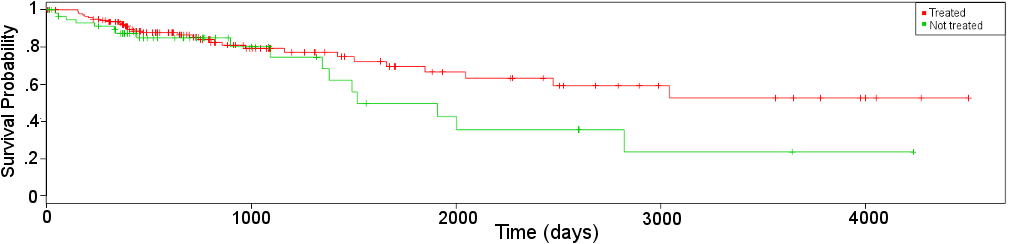
\includegraphics[scale=0.4]{images/example_kaplan_meier_curve}
	\caption{Voorbeeld kaplan-meier survival curves. De X-as geeft de tijd weer, de Y-as geeft de kans weer op overleving.}
	\label{fig:D:cox-example-kaplan-meier}
\end{figure}
Bij overlevingsanalyze wordt echter ook vaak gebruik gemaakt van de zogenaamde hazard (of risico) functie. Deze functie geeft weer wat het risico is dat op een gegeven tijdstip het event zich voordoet. In het cox proportionele risico model dat we zullen gebruiken wordt deze risico functie als volgt genoteerd:
\begin{equation}
\begin{split}
\lambda_{i}(t) = \lambda_{0}(t)e^{X_{i1}\beta_{1} + ... + X_{iN}\beta_{N}}
\end{split}
\end{equation}
where
\begin{itemize}
	\item $\lambda_{i}(t)$ is het risico op overlijden voor pati\"ent i op tijdstip t.
	\item $\lambda_{0}(t)$ is de baseline risico op tijdstip t, dit is het risico op overlijden zonder enige invloed van de input variabelen.
	\item $X_{i1} ... X_{iN}$ zijn de waarden voor de input variabelen voor pati\"ent i.
	\item $\beta_{1} ... \beta_{N}$ zijn de waarden voor de parameters van het model (de kennis representatie).
\end{itemize}
Een tweede interessant concept is wat met noemt de risico-verhouding (hazard ratio). Dit is de verhouding van twee risico functies:
\begin{equation}
\label{eq:D:cox-hazard-ratio}
\begin{split}
\frac{\lambda_{i}(t)}{\lambda_{j}(t)} 
= \frac{\lambda_{0}(t)e^{X_{i1}\beta_{1} + ... + X_{iN}\beta_{N}}}{\lambda_{0}(t)e^{X_{j1}\beta_{1} + ... + X_{jN}\beta_{N}}}
= e^{(X_{i1}-X_{j1})\beta_{1} + ... + (X_{iN}-X_{jN})\beta_{N}}
\end{split}
\end{equation}
Merk op dat de vorm van de risico functie een keuze is die we zelf hebben gemaakt, door te kiezen voor cox proportionele risico modellen. Deze keuze heeft twee heel belangrijke gevolgen die duidelijk worden in de formule van de risico-verhouding (\ref{eq:D:cox-hazard-ratio}). Het eerste gevolg is dat risico-verhoudingen onafhankelijk zijn van de tijd. Dit wil zeggen dat de risico-verhouding tussen twee pati\"nten dus niet verandert doorheen de tijd. Vandaar ook de naam 'proportionele risico modellen'. Het tweede gevolg is dat veranderingen in de input variabelen een multiplicatief effect hebben op het risico. Dit kunnen we ook zien in formule \ref{eq:D:cox-hazard-ratio}, maar is nog duidelijker als we de risico-verhouding neerschrijven met in de noemer het risico voor een pati\"ent met bepaalde waarden voor de input variabelen, en in de teller het risico voor een pati\"ent met exact dezelfde input waarden, behalve voor 1 variabele $X_{j}$ een verhoging met 1:
\begin{equation}
\begin{split}
\frac{\lambda(t|X_{j}+1)}{\lambda(t|X_{j})} = e^{(X_{j}+1-X_{j})\beta_{j}} = e^{\beta_{j}}
\end{split}
\end{equation}
We zien dus dat een verhoging met 1 voor een input variabele, het risico doet veranderen met $e^{\beta_{j}}$, de exponenti\"ele van de bijhorende co\"effici\"ent.

\subsubsection{Het predictief overlevingsmodel}
Net zoals bij logistieke regressie hebben we hier dus te maken met een set gewichten die onze kennis representatie voorstellen. We zullen ook heel analoog een iteratief algoritme gebruiken om deze gewichten te bepalen. We zullen het model een hele reeks voorbeeld datapunten tonen (input variabelen met bijhorende overlevingskans) om zo het model ervaring te laten opbouwen en op die manier zo goed mogelijk de overlevingskansen van pati\"enten te laten schatten.

\subsection{Regularizatie}
Een belangrijk concept dat we moeten toevoegen aan onze modellen is regularizatie. Herinner je uit sectie \ref{sec:D:pm} dat we een predictief model opbouwen door het een reeks voorbeeld datapunten te geven om het op die manier zijn interne representatie van de kennis te laten opbouwen. In beide voorbeeld modellen die we hebben gezien is deze representatie en set van gewichten. Het concept van regularizatie houdt in dat we een of meerdere beperkingen gaan opleggen aan deze gewichten. Het doel hiervan is om bepaalde modellen (bepaalde combinaties van gewichten) te prefereren boven anderen. De onderliggende gedachte is dat we gaan trachten van simpele modellen te bekomen, die een vloeiende functie voorstellen. We doen dit om te voorkomen dat het model patronen gaat vinden die er eigenlijk niet zijn of die enkel het resultaat zijn van ruis is de gegevens. Er zijn verschillende beperkingen mogelijk die we kunnen opleggen, en elk krijgen ze hun eigen naam: de ridge penalty, de lasso penalty en het elastisch-net pentalty.
\subsubsection{Ridge penalty}
Bij de ridge penalty (ook wel $L_{2}$ panalty genoemd) is de beperking die we opleggen de volgende:
$$
\sum_{i=1}^{N}w_{i}^{2} \leq C
$$
Deze beperking zal ervoor zorgen dat gewichten klein worden gehouden, en het dus onmogelijk wordt dat een gewicht extreem groot wordt relatief ten opzichte van de andere gewichten.
\subsubsection{Lasso penalty}
Bij de lasso penalty (ook wel $L_{1}$ penalty genoemd) is de beperking:
$$
\sum_{i=1}^{N}\lvert w_{i}\rvert \leq C
$$
Deze beperking heeft ook als gevolg dat de gewichten klein worden gehouden, maar heeft als extra dat gewichten ook effectief 0 worden indien ze niet belangrijk genoeg zijn in het model. We noemen dit daarom ook 'variabele selectie'. Gebruik van de lasso penalty heeft als gevolg dat het resulterende model vaak minder parameters gebruikt, omdat het enkel deze parameters gebruikt die echt belangrijk zijn. Deze techniek zal zeer belangrijk blijken bij een van de integratie technieken die later worden besproken.
\subsubsection{Elastisch-net penalty}
Bij het elastisch-net penalty is de beperking een combinatie van de ridge en lasso penalties:
$$
\alpha \sum_{i=1}^{N}w_{i}^{2} + (1-\alpha)\sum_{i=1}^{N}\lvert w_{i}\rvert \leq C
$$
Deze methode heeft daarom ook eigenschappen van zowel ridge als lasso, en met de parameter $\alpha$ kan men kiezen hoezeer men wil aanleunen bij een van de twee technieken. Dit vormt als het ware een gulden middenweg.
\subsubsection{De parameter $\lambda$}
Wanneer met regularizatie echter toepast op een concreet model, zal men altijd het optimalisatie probleem met beperking proberen omvormen naar een equivalent optimalisatie probleem zonder beperking. Bij deze omvorming introduceert men dan meestal een parameter $\lambda$ die als vervanging dient voor de parameter $C$ in bovenstaande beperkingen. $\lambda$ kan men zien als de hoeveelheid regularizatie die men wil gebruiken. Hoe groter $\lambda$ hoe sterker de beperking en dus hoe kleiner $C$. Hoe kleiner $\lambda$, hoe minder regularizatie, hoe groter $C$.

\subsection{Validatie}
Het laatste concept dat we moeten behandelen is validatie. Dit zal ons toelaten om een getraind model te evalueren. Bij validatie delen we onze dataset op in twee delen: een training set en een validatie set. De training set kennen we reeds, deze datapunten zullen we gebruiken om een model te trainen. Merk op dat we nu echter nog datapunten over hebben die niet gebruikt werden voor de training, dit is de validatie set. We zullen het getrainde model vragen om voor deze datapunten een predictie te berekenen voor de output variabelen. We kennen van de datapunten in de validatie set echter de correcte output waarde. We kunnen vervolgens dus de output van ons predictief model vergelijken met de juiste waarde, en op die manier een idee krijgen hoe goed ons predictief model presteert. \\ \\
Merk echter op dat de training set die we gebruiken om het model te trainen kleiner is dan de volledige dataset waarover we beschikken. We houden inderdaad de datapunten in de validatie set opzij. We willen echter zoveel mogelijk datapunten gebruiken om te trainen, want dan bekomen we een beter model. Langs de andere kant willen we ook genoeg datapunten in de validatie set om een goed beeld te krijgen van de performantie van het bekomen model. Een oplossing voor deze contradictie is cross-validatie. Bij cross-validatie delen we onze dataset op in K (vaak 10) gelijke stukken. We gebruiken 1 van de K stukken als validatie set, en de andere K-1 stukken als training set. We herhalen dit proces K keren, waarbij we iedere keer een ander stuk nemen als validatie set. Op die manier hebben we op het einde voor elk datapunt in onze dataset een predictie. Deze predicties kunnen we dan vergelijken met de echte waarden en dit zal ons een redelijk goed beeld geven van de performantie van het model dat we zouden bekomen indien we op de volledige dataset zouden trainen.

\section{Integratie technieken}
\label{cha:D:integratie}

\subsection{Inleiding}
\label{sec:D:integratie-inleiding}
In dit hoofdstuk stellen we drie verschillende integratie technieken voor. Eerst zullen we kort overlopen hoe de data eruit ziet waar we van vertrekken, en vervolgens zullen we de drie technieken overlopen. De eerste strategie noemen we vroege-integratie en is gebaseerd op het aan elkaar voegen van datasets. De tweede strategie heet late-integratie en is gebaseerd op het concept van 'ensemble-learning'. De laatste techniek heet parti\"ele integratie en maakt gebruik van de variabele selectie in de lasso regularizatie. 

\subsection{Beschrijving van de data}
\label{sec:D:integratie-beschrijving}
Integratie duidt op het combineren van verschillende elementen. In dit geval zijn de elementen waarmee we te maken hebben datasets. Herinner je dat we, om een model te trainen, een lijst van gelabelde datapunten nodig hadden. Zo een lijst noemen we een dataset. Nu hebben we te maken met meerdere datasets, en moeten we een strategie bedenken om deze verschillende datasets te gebruiken om een model te trainen. Merk op dat het noodzakelijk is om datapunten over verschillende datasets aan elkaar te koppelen. Met andere woorden, alle datapunten in de datasets moeten een vorm van unieke identificatie krijgen waardoor we gegevens van verschillende datasets, die spreken over eenzelfde datapunt, aan elkaar kunnen koppelen.

\subsection{Vroege integratie}
\label{sec:D:integratie-vroeg}
Bij vroege integratie gaan we op voorhand (voor het trainen) alle gegevens over eenzelfde datapunt aan elkaar koppelen. Dit is mogelijk omdat elk datapunt een unieke identificatie krijgt. We kunnen dit bezien als het aan elkaar plakken van alle datasets, waardoor we uiteindelijk overblijven met slechts $\acute{e}\acute{e}n$ grotere dataset. Een schematisch overzicht van vroege integratie wordt gegeven op figuur \ref{fig:D:integratie-vroeg}.
\begin{figure}
	\centering
	\includegraphics[scale=.8]{images/early_integration}
	\caption{Schema voor vroege integratie}
	\label{fig:D:integratie-vroeg}
\end{figure}

\subsection{Late integratie}
\label{sec:D:integratie-laat}
Bij late integratie zullen we eerst voor elke dataset apart een model trainen. Als het aantal datasets gelijk is aan $D$ dan zullen we dus ook $D$ predictieve modellen bekomen. Wanneer we dan voor een nieuw (ongezien) datapunt een predictie moeten maken, zullen we dit datapunt aan elk van de $D$ predictieve modellen geven. Zij zullen elk individueel een predictie maken. Vervolgens combineren we de $D$ voorspelde waarden in een lineaire combinatie om tot een finale predictie waarde te komen. Indien we geen extra waarde willen hechten aan een van de $D$ modellen kunnen we voor deze lineaire combinatie gewoon het gemiddelde nemen van alle voorspelde waarden. \\ \\
In het veld van machine-leren is het concept van ensemble-leren reeds bekend. Dit houdt in dat voor een bepaald probleem meerdere verschillende modellen worden getraind op dezelfde dataset. Het combineren van de output van de verschillende modellen kan dan een beter resultaat geven vergeleken met een enkel model. Dit komt doordat de verschillende modellen mogelijks fouten maken op verschillende vlakken, en door uitmiddeling van de outputs worden deze fouten relatief verkleint. De late integratie techniek neemt deze gedachtengang over. We gebruiken nu niet meerdere modellen voor dezelfde dataset, maar we gebruiken meerdere modellen voor meerdere datasets. Door deze uitmiddeling hopen we echter eenzelfde foutenreductie te bekomen. Een schematisch overzicht van de late integratie techniek wordt getoond op figuur \ref{fig:D:integratie-laat}.
\begin{figure}
	\centering
	\includegraphics[scale=.8]{images/late_integration}
	\caption{Schema voor late integratie}
	\label{fig:D:integratie-laat}
\end{figure}

\subsection{Parti\"ele integratie}
\label{sec:D:integratie-partieel}
De laatste methode die we voorstellen is de parti\"ele integratie. Deze methode vertrekt analoog aan de late integratie door voor elke dataset individueel een predictief model op te stellen. Belangrijk hierbij is op te merken dat bij het trainen van deze modellen de lasso regularizatie wordt gebruikt. Dit doen we om gebruik te maken van de variabele selectie eigenschap. Door deze variabele selectie zullen de resulterende modellen ons namelijk vertellen welke variabelen zij belangrijk achten in de datasets. De volgende stap is dan om uit elke dataset enkel die variabelen te extraheren die door de modellen geselecteerd werden. Deze geselecteerde gegevens worden dan aan elkaar geplakt zoals in de vroege integratie, op basis van unieke identificatie van de datapunten. Dit geeft ons een nieuwe, gereduceerde, dataset. Deze dataset gebruiken we vervolgens om opnieuw een predictief model op te stellen, dit is het finale ge\"integreerde model dat we zullen gebruiken voor predictie. Merk op dat deze techniek dus in twee stappen werkt, er zijn twee training fases. Een schematische voorstelling van de parti\"ele integratie wordt gegeven op figuur \ref{fig:D:integratie-partieel}.

\begin{figure}
	\centering
	\includegraphics[scale=.8]{images/intermediate_integration}
	\caption{Schema voor parti\"ele integratie}
	\label{fig:D:integratie-partieel}
\end{figure}

\section{Evaluatie van integratie methoden}
\label{cha:D:evaluatie}

\subsection{Introductie}
\label{sec:D:evaluatie-introductie}
In dit hoofdstuk zullen we onderzoeken of de verschillende integratie strategie\"en en impact hebben op de performantie van de resulterende modellen. We doen dit door in twee concrete case studies, op echte kankergegevens, een model uit te werken gebruikmakend van elke strategie. En vervolgens de bekomen modellen te evalueren met een passende metriek.

\subsection{Case studie 1: logistieke regressie}
\subsubsection{Case overzicht}
In de eerste case studie zullen we logistieke regressie modellen gebruiken. De gebruikte datasets komen van het Universitair Ziekenhuis te Leuven en betreffen gegevens van pati\"enten met darmkanker. Van deze pati\"enten zijn tijdens de behandeling scans genomen met een MRI scanner, PET scanner en DWI scanner. We hebben in dit geval dus te maken met drie datasets. De output variabele die we zullen trachten te voorspellen is een binaire versie van het pathologisch stadium van elke pati\"ent (zie appendix \ref{app:cancer-staging}). We kunnen stellen dat pati\"enten met een label 1 van de kanker zijn genezen, en pati\"enten met een label 0 niet. Deze output die het predictief model ons zal geven is dus een kans op genezing.
\subsubsection{Evaluatie methode}
We zullen de logistieke modellen evalueren met een Receiver-Operator Characteristic analyse. Herinner je dat we via cross-validatie voor elk datapunt in onze dataset een predictie konden bekomen. In het geval van logistieke regressie is deze predictie een probabiliteit. De output voor de datapunten in onze dataset zijn echter binaire waarden (de realisaties van de binomiaalverdeling). Om de twee te kunnen vergelijken moeten we een drempelwaarde defini\"eren. Als de voorspelde probabiliteit hoger is dan deze drempelwaarde dan voorspellen we een positieve output, anders een negatieve output. Voor elk datapunt zijn er hierbij dan vier scenario's mogelijk:
\begin{itemize}
	\item True Positive (TP): het model voorspelt een positieve output, en dat is correct
	\item True Negative (TN): het model voorspelt een negatieve output, en dat is correct
	\item False Positive(FP): het model voorspelt een positieve output, en dat is fout (type 1 fout)
	\item False Negative (FN): het model voorspelt een negatieve output, en dat is fout (type 2 fout)
\end{itemize}
Merk op dat we in dit geval niet enkel zeggen of het model juist of fout was, maar ook de type fout registreren. Dit laat ons toe om volgende begrippen van sensitiviteit en specificiteit te defini\"eren:
$$
sensitiviteit = \frac{\sum{TP}}{\sum{P}}
$$
$$
specificiteit = \frac{\sum{TN}}{\sum{N}}
$$
hierin zijn
\begin{itemize}
	\item $\sum{TP}$ het totale aantal true positives
	\item $\sum{P}$ is het totale aantal datapunten met positieve output in de dataset
	\item $\sum{TN}$ het totale aantal true negatives
	\item $\sum{N}$ is het totale aantal datapunten met negatieve output in de dataset
\end{itemize}
Het perfecte model, dat altijd juist voorspelt, heeft een sensitiviteit en specificiteit gelijk aan 1. In een realistische setting is dit echter zelden haalbaar. We willen beide metrieken echter zo dicht mogelijk bij 1. We kunnen nu een plot maken waarbij we op de sensitiviteit plotten in functie van de specificiteit voor verschillende waarden van de drempelwaarde. Merk op dat inderdaad verschillende drempelwaarden ervoor zullen zorgen dat het model verschillende voorspellingen maakt en dus sensitiviteit en specificiteit zullen be\"invloeden. De curve die we bekomen op deze plot noemt men een Receiver Operating Characteristic curve. Een voorbeeld curve wordt getoont op figuur \ref{fig:D:evaluation-roc}. De metriek die we zullen gebruiken is de oppervlakte onder deze ROC curve, ook wel afgekort AUC(Area Under the ROC Curve). Hoe hoger deze waarde, hoe groter de waarden voor sensitiviteit en specificiteit bij verschillende drempelwaarden, en dus hoe beter ons predictief model.
\begin{figure}
	\centering
	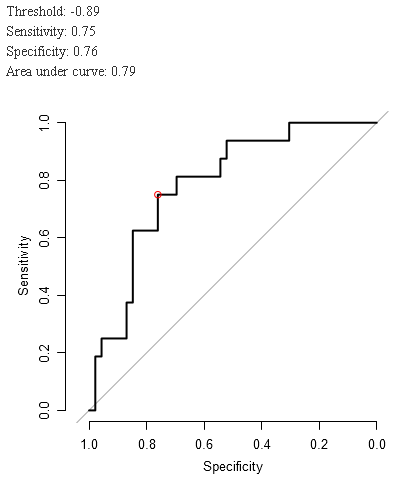
\includegraphics[scale=.7]{images/roc_curve}
	\caption{Voorbeeld ROC curve en metrieken}
	\label{fig:D:evaluation-roc}
\end{figure}

\subsection{Resultaten}
De resulterende AUC waarden worden getoond in tabellen \ref{tab:D:evaluation-auc-individual} en \ref{tab:D:evaluation-auc-integrated}, respectievelijk voor modellen op individuele datasets, en ge\"integreerde modellen.
Uit de eerste tabel is het duidelijk dat de MRI dataset de meeste predictieve informatie bevat. Maar door gebruik te maken van integratie technieken kunnen we duidelijk de performantie van de modellen verbeteren. Tevens kunnen we opmerken dat, onafhankelijk van de gebruikte datasets, de parti\"ele integratie de beste methode blijkt in dit geval.
\begin{table}
	\centering
	\begin{tabular}{lc}
		\toprule
		Dataset & AUC \\
		\midrule
		DWI & 0.67 \\
		MRI & 0.75 \\
		SUV & 0.65 \\
		\bottomrule
	\end{tabular}
	\caption{AUC voor modellen getraind op individuele datasets}
	\label{tab:D:evaluation-auc-individual}
\end{table}
\begin{table}
	\centering
	\begin{tabular}{lcccc}
		\toprule
		& Alle datasets & DWI+MRI & DWI+SUV & MRI+SUV \\
		\midrule
		Vroege integratie & 0.76 & 0.82 & 0.69 & 0.74 \\
		Parti\"ele integratie & 0.79 & 0.83 & 0.78 & 0.75 \\
		Late integratie & 0.73 & 0.78 & 0.66 & 0.70 \\
		\bottomrule
	\end{tabular}
	\caption{AUC voor ge\"integreerde modellen voor verschillende combinaties van de datasets}
	\label{tab:D:evaluation-auc-integrated}
\end{table}
\subsection{Case studie 2: cox proportionele risico modellen}
\subsubsection{Case overzicht}
In de tweede case studie zullen we cox modellen gebruiken. De gebruikte datasets komen in dit geval van The Cancer Genome Atlas. Dit is een project van het National Cancer Institute waarbij 2.5 petabytes aan gegevens werden publiek gemaakt over pati\"enten met 33 types van kanker. Hiervan zullen we gebruik maken van enkele datasets voor keelkanker pati\"enten. Meerbepaald de datasets met Copy Number Variaties, messenger RNA data en micro RNA data. Dit zijn drie datasets die aanwijzingen geven over defecten in het DNA. We zullen deze gegevens proberen te correleren met de overlevingskans van pati\"enten gebruikmakend van het cox model.
\subsubsection{Evaluatie methode}
Om de overlevingsmodellen te evalueren zullen we gebruik maken van een significantie test genaamd de Wald Test. Een significantie test vergelijkt het bekomen model met een ander hypothetisch model genaamd de null-hypothese. In dit geval is de null-hypothese het overlevingsmodel waarbij alle gewichten (de parameters van ons model) gelijk zijn aan 0. Dit zou willen zeggen dat geen enkele van de variabelen in de datasets een impact heeft op de overleving (of op het risico tot overlijden) van de pati\"enten. Een significantie-test is bedoeld om aan te tonen dat deze null-hypothese te verwerpen is, namelijk dat de gegevens die geobserveerd worden heel erg onwaarschijnlijk zijn, in het geval dat de null-hypothese waar is. Als we die onwaarschijnlijkheid kunnen aantonen dan zeggen we dat we de null-hypothese verwerpen, en dat geeft aan dat het model dat we gevonden hebben significant is. De formule voor de Wald test waarbij 1 enkele variabele wordt getest is:
\begin{equation}
\begin{split}
\frac{(\hat{\beta}-\beta_{0})^{2}}{var(\hat{\beta})} \sim \tilde{\chi}^{2}_{1}
\end{split}
\end{equation}
where
\begin{itemize}
	\item $\hat{\beta}$ is de waarde voor de variabele die we zijn bekomen in ons model
	\item $\beta_{0}$ is de waarde van de variabele $\beta$ indien de null-hypothese waar is, in ons geval is dat de waarde 0.
	\item $var(\beta)$ is de variantie van de variabele $\beta$
	\item $\tilde{\chi}^{2}_{1}$ is de chi-kwadraat verdeling met 1 vrijheidsgraad
\end{itemize}
Wat de Wald test dus berekent is de afstand tussen de gevonden waarde, en de waarde onder de null-hypothese, relatief ten opzichte van de onzekerheid over de variabele (de variantie). Hoe groter de waarde van de Wald test, hoe significanter het model. Een schematische voorstelling wordt gegeven op figuur \ref{fig:D:evaluation-wald-test}. In de statistiek wordt deze waarde echter vaak omgevormd tot een p-waarde. De p-waarde is een waarde tussen 0 en 1 (het is een probabiliteit), en is berekenbaar uit de waarde van de Wald test. Het geeft dus geen enkele extra toegevoegde waarde, maar we tonen deze waarde omwille van zijn populariteit. Daarnaast is het ook veelvoorkomend om een drempelwaarde in te stellen voor de p-waarde. Indien de p-waarde lager ligt dan deze waarde beschouwen we het model als significant. Een veelgebruikte drempelwaarde is 0.05.
\begin{figure}
	\centering
	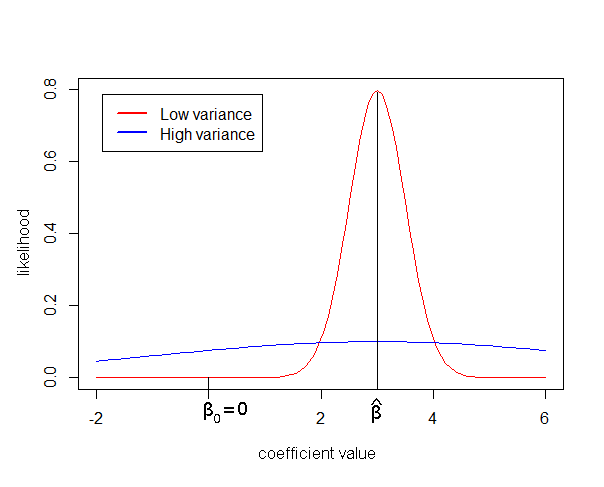
\includegraphics[scale=.7]{images/wald_test}
	\caption{Voorbeeld Wald test variantie visualisatie. Beide curves geven dezelfde maximum likelihood schatting voor $\hat{\beta}$. De rode curve heeft echter een lage variantie, wat veel evidentie biedt om de null-hypothese te verwerpen. De blauwe curve heeft een hoge variantie, in dit geval is het niet meteen duidelijk dat $\hat{\beta}$ echt verschilt van $\beta_{0}$ en dus kunnen we de null-hypothese niet verwerpen.}
	\label{fig:D:evaluation-wald-test}
\end{figure}

\subsection{Resultaten}
Tabel \ref{tab:D:evaluation-case2-dimensions} geeft een overzicht van de dimensies van de gebruikte datasets. De resultaten van de significantietests voor alle modellen worden getoond in de tabellen \ref{tab:D:evaluation-surv-individual} en \ref{tab:D:evaluation-surv-integrated}. Het is meteen duidelijk dat bijna alle modellen niet significant zijn. De berekende p-waarden zijn duidelijk ver boven de vooropgestelde grens van 0.05. Dat terzijde is het interessant om op te merken dat alle ge\"integreerde modellen duidelijk meer significant zijn dan de modellen voor individuele datasets. Meer nog, het partieel ge\"integreerde model is het enige model dat het significantie niveau van 0.05 bereikt. Er zou echter meer onderzoek moeten gebeuren om de werkelijke predictieve waarde van dit model te onderzoeken, maar voor deze studie is het duidelijk dat dit model het beste model is. En dus kunnen we concluderen dat de ge\"integreerde modellen ook hier aantonen dat ze een positieve impact hebben op de performantie van de bekomen modellen.
\begin{table}
	\centering
	\begin{tabular}{lcc}
		\toprule
		Dataset naam & Aantal variabelen & Aantal pati\"enten \\
		\midrule
		Copy Number Variations & 16 & 219\\
		messenger RNA & 3869 & 219 \\
		micro RNA & 414 & 219 \\
		\bottomrule
	\end{tabular}
	\caption{Dimensies voor de datasets die gebruikt werden in de overlevingsanalyse.}
	\label{tab:D:evaluation-case2-dimensions}
\end{table}

\begin{table}
	\centering
	\begin{tabular}{lccc}
		\toprule
		& CNV    & mRNA & miRNA \\
		\midrule
		Wald test 					& 0.17 & 0.13  & 1.46 \\
		P-waarde 					& 0.6799 & 0.7209  & 0.2276 \\
		\bottomrule
	\end{tabular}
	\caption{Significantie waarden voor de overlevingsmodellen voor individuele datasets}
	\label{tab:D:evaluation-surv-individual}
\end{table}

\begin{table}
	\centering
	\begin{tabular}{lccc} 
		\toprule
		& Early & Intermediate & Late\\
		\midrule
		Wald test 					& 2.43 & 3.89 & 1.98 \\
		P-waarde 					& 0.1192 & 0.0485 & 0.1595 \\
		\bottomrule
	\end{tabular}
	\caption{Significantie waarden voor de ge\"integreerde overlevingsmodellen}
	\label{tab:D:evaluation-surv-integrated}
\end{table}

\section{Conclusie}
\label{cha:D:conclusie}
Het eerste hoofdstuk toont aan dat er een nood is aan data-integratie methoden door de steeds groeiende datasets waarmee we moeten werken. Door op een slimme manier verschillende datasets te integreren kunnen we predictieve modellen bouwen die beter presteren. \\ \\
Vervolgens beschreven we wat predictieve modellen inhouden en we toonden twee concrete voorbeelden: logistieke regressie - en cox modellen.  \\ \\
Met deze informatie konden we vervolgens de verschillende integratie strategi\"en voorstellen. De eerste strategie, vroege integratie, voegt alle datasets aan elkaar door overeenkomende datapunten te linken. De tweede strategie, late integratie, bouwt individuele modellen voor elke dataset, ge\"inspireerd op het concept van ensemble-leren. De laatste strategie, parti\"ele integratie, bouwt het predictief model in twee stappen en maakt gebruik van de variabele selectie eigenschap in de lasso regularisatie. \\ \\
Om aan te tonen dat de verschillende integratie strategie\"en een impact hebben op de performantie van de predictieve modellen, passen we de strategie\"en toe in twee case studies met echte gegevens over kankerpati\"enten. De eerste studie gebruikt logistieke regressie modellen. De data voor deze studie komt van het Universitair Ziekenhuis te Leuven en betreft scan-gegevens voor pati\"enten met darmkanker. De resultaten van deze studie tonen een duidelijke verbetering van de performantie door het gebruik van integratie. De tweede case studie gebruikt cox proportionele risico modellen. De data van deze studie kwam van de online TCGA database. De resultaten in deze studie waren minder evindent, maar we kunnen toch besluiten dat ook in dit geval de ge\"integreerde modellen beter presteren dan de individuele modellen. En specifiek het partieel ge\"integreerde model bleek het beste te zijn. Beide studies leveren daarom evidentie aan dat integratie van datasets inderdaad de performantie ten goede komt, en dat verschillende strategie\"en een verschillende impact hebben. \\ \\
Het moet echter duidelijk zijn dat dit niet het einde van de studie is. In dit thesis toonden we drie verschillende integratie strategie\"en, maar er zijn duidelijk nog veel andere manier mogelijk om datasets te integreren. Verder spitste de case studies in dit geval zich toe op twee lineaire modellen: logistieke regressie- en cox modellen. Een interessante uitbreiding is om te kijken of deze claims ook gelden voor andere (niet-lineaire) methoden. \\ \\
Daarnaast moeten we in ons achterhoofd onthouden dat deze studie kadert in een grotere studie wiens doel het is om patronen en nieuwe inzichten te vinden in de grote hoeveelheden kankergegevens waarover we beschikken. Door betere predictieve modellen te bouwen kunnen we in de toekomst nieuwe inzichten verkrijgen in de manier waarop kankers ontstaan en zich ontwikkelen. Dit zal op zijn beurt in de toekomst een weg bieden naar nieuwe behandelingen voor kanker.


\end{abstract*}

%%% Local Variables: 
%%% mode: latex
%%% TeX-master: "thesis"
%%% End: 

	
	\backmatter
	% Na de bijlagen plaatst men nog de bibliografie.
	% Je kan de  standaard "abbrv" bibliografiestijl vervangen door een andere.
	\bibliographystyle{abbrv}
	\bibliography{references}
	
\end{document}

%%% Local Variables: 
%%% mode: latex
%%% TeX-master: t
%%% End: 
